\documentclass[11pt,twoside]{book}

% --- Engine-agnostic fonts, per house convention: LuaLaTeX + TeX Gyre Pagella ---
\usepackage{fontspec}
\setmainfont{TeX Gyre Pagella}

\usepackage[margin=1.15in]{geometry}
\usepackage{amsmath}
\usepackage{amssymb}
\usepackage{longtable}
\usepackage{booktabs}
\usepackage{array}
\usepackage{calc}
\providecommand{\real}[1]{#1}
\usepackage{tikz}
\usetikzlibrary{arrows.meta,positioning,calc,matrix,decorations.pathreplacing}
\usepackage{pgfplots}
\pgfplotsset{compat=1.18}
\usepackage{enumitem}
\usepackage[dvipsnames]{xcolor}
\usepackage[colorlinks=true,linkcolor=Maroon,urlcolor=Maroon,citecolor=Maroon]{hyperref}
\usepackage{titlesec}
\usepackage{fancyhdr}
\usepackage{microtype}

% Chapter/part styling: understated, matching continuous-academic-prose convention
\titleformat{\part}[display]{\normalfont\Large\itshape\centering}{Part \Roman{part}}{1em}{\Huge\bfseries}
\titleformat{\chapter}[display]{\normalfont\bfseries}{}{0pt}{\Large}

\pagestyle{fancy}
\setlength{\headheight}{14pt}
\fancyhf{}
\fancyhead[LE,RO]{\thepage}
\fancyhead[RE]{\nouppercase{\leftmark}}
\fancyhead[LO]{\nouppercase{\rightmark}}
\renewcommand{\headrulewidth}{0.4pt}

% Long-table continuation headers used by pandoc output
\providecommand{\tightlist}{\setlength{\itemsep}{0pt}\setlength{\parskip}{0pt}}

\title{\bfseries Contradiction and Continuation:\\[0.3em]
\large A Constraint-Theoretic Derivation of Non-Classical Logic}
\author{Flyxion \\ \normalsize Independent Researcher}
\date{2026}

\begin{document}

\frontmatter

\maketitle

\tableofcontents

\hypertarget{front-matter}{%
\label{front-matter}}

\hypertarget{abstract}{%
\chapter*{Abstract}
\addcontentsline{toc}{chapter}{Abstract}
\markboth{Abstract}{Abstract}\label{abstract}}

This book sets out to derive Graham Priest's non-classical and dialetheic
logics from a general theory of constrained representation, rather than
presenting classical logic as the default and non-classical systems as
deviations from it. It does not deliver the result it initially expected.
Early planning aimed at a Glut--Obstruction Correspondence: some precise
identification of Priest's contradictions with a geometric obstruction to
assembling local evidence into a coherent whole. The completed manuscript
establishes close to the opposite, and the result generalizes past the
one theorem it was first stated for: \textbf{contradiction and obstruction are
independent facts about the same data.} Chapter 22's Mutual
Non-Determination Proposition is this claim's sharpest instance --- whether
a proposition is contradictory and whether its supporting evidence
coheres do not determine one another, and an explicit six-cell
construction proves it rather than merely failing to disprove it --- but
the same pattern recurs throughout the book: apparently related
structures are repeatedly shown to carry independent coordinates rather
than collapsing into one. Three further correspondences investigated
with equal seriousness --- non-normal worlds as refusal, bilattice merge as
ordinary sheaf gluing, glut as a nonzero cohomology class --- were rejected
outright, at three different structural levels (modal, operational,
geometric), after being plausible enough to have been provisionally
accepted earlier in the project. The book's actual thesis, assembled from
these results rather than imposed on them in advance, is that
non-classical logics need not be understood as competing relaxations of
one classical standard; they can be understood as responses to different
failures along structural axes that turn out, on inspection, to be
substantially independent of one another.

\hypertarget{introduction}{%
\chapter*{Introduction}
\addcontentsline{toc}{chapter}{Introduction}
\markboth{Introduction}{Introduction}\label{introduction}}

\hypertarget{what-this-book-does-not-do}{%
\section{What this book does not do}\label{what-this-book-does-not-do}}

It does not treat classical logic as the ground state from which
paraconsistent, intuitionistic, relevant, many-valued, and modal systems
are departures requiring justification. Chapter 1 states the alternative
directly: logical consequence is preservation under admissible
transformation, \(x \leadsto_R y\), with classical logic sitting at one
specific point in the space of possible regimes \(R\) --- the point
combining maximal strictness on valuation (no gaps, no gluts) with
unrestricted explosive propagation from contradiction under the relevant
closure principles. Every other logic covered in this book is a
different point in the same space --- an alternative regime whose adequacy
depends on the constraints governing the representational task at hand,
not an equally good option regardless of task, and not a weakening of
the classical one. Admissibility is precisely what lets the book
discriminate among regimes; nothing here is an argument for treating all
regimes as interchangeable.

By the book's own account, this way of stating things is only earned
because three plausible correspondences failed to survive their
chapters: non-normality is not refusal, merge is not gluing, and glut is
not obstruction. A reader should not expect a book that translates every
Priest concept into this framework's vocabulary and declares victory ---
several translations were attempted and explicitly rejected, and that
outcome is treated as evidence for the book's thesis rather than as
incidental failure.

\hypertarget{the-question-the-book-actually-asks}{%
\section{The question the book actually asks}\label{the-question-the-book-actually-asks}}

Stated once, in Chapter 1, and returned to throughout: \emph{what must remain
invariant when representations are combined, transported, refined,
contradicted, or extended?} This is deliberately not the question
``which logic is correct.'' It's a question about which structural
distinctions survive contact with an actual formal system, once that
system is built rather than merely proposed.

\hypertarget{separation-before-unification}{%
\section{Separation before unification}\label{separation-before-unification}}

The book's method, visible in retrospect across all six parts, is to
take something ordinarily treated as one notion and ask whether it's
actually several. Nearly every chapter that matters does this. Chapter 6
separates admissibility and accessibility: what states a regime permits,
versus which of those states a given world can modally reach. Chapter 7
separates inconsistency, impossibility, and non-normality: a state
containing a contradiction, a state failing to satisfy a governing
regime, and a state whose evaluation rules are themselves suspended are
three independent facts, not one phenomenon under three names. Chapters
9 and 10 separate positive and negative support: the two questions ``is
there evidence for'' and ``is there evidence against,'' whose four
possible joint answers generate Belnap and Dunn's four truth values as a
consequence rather than a stipulation. Chapter 13 separates support and
constructibility: whether evidence exists, and whether it takes the
specific form of an exhibitable witness, answer different questions even
when the same proposition is at issue. Chapters 15 and 20--21 separate
compatibility and dispersion: local evidence disagreeing outright, versus
locally negligible variation that nonetheless accumulates past a
threshold under coarse-graining, are different failure mechanisms with
different mathematics. Chapters 20--22 separate semantic glut from
geometric coherence defect: a proposition's contradictory support status,
and whether the evidence behind that status agrees with itself across
overlapping contexts, do not determine one another. Chapters 20--21
separate gluing, merge, and repair: reconstructing a section from a
family that already agrees, versus combining a family that doesn't agree
while retaining everything it supplied, are different operations that an
earlier draft of this project once conflated under one word.

None of these separations were chosen for elegance in advance. Several
were forced by a correspondence failing to hold up once its chapter was
actually drafted --- recorded, not smoothed over, in the correspondence
ledger this book's technical claims are checked against.

\hypertarget{the-hierarchy-this-produces}{%
\section{The hierarchy this produces}\label{the-hierarchy-this-produces}}

Six questions, asked of the same underlying material at increasing
levels of structure, form the closest thing this book has to a single
conceptual synopsis:

\[\text{support} \to \text{construction} \to \text{compatibility} \to \text{repair} \to \text{persistence} \to \text{continuation}.\]

Does evidence exist? Can it be exhibited? Can local descriptions coexist?
If not, can they be minimally reconciled without discarding either? Does
the resulting determination survive a change of scale? Does it remain
identifiable as the same thing through a change of state? These are
successive questions in the book's analysis, asked in this order because
each becomes askable once the last has been separated out --- not because
each presupposes or reduces to the one before it. Construction does not
intrinsically presuppose support, and compatibility does not
intrinsically presuppose construction; the book argues for their
independence rather than building a reduction chain. The six parts
largely track this order, though not in the sequence they were drafted.

\hypertarget{the-parameter-that-becomes-structure}{%
\section{The parameter that becomes structure}\label{the-parameter-that-becomes-structure}}

There's a second way to see the same six parts, sharper for being purely
technical: watch what happens to the single parameter \(R\) introduced in
Chapter 1.

\[R \to (R, \mathcal{R}) \to (R, \mathcal{R}, \sigma^+, \sigma^-) \to \text{local support/coherence} \to \text{repair and persistence} \to R_w\text{-dependent continuation}.\]

Chapter 1 treats admissibility as one relation governing consequence.
Chapter 6 finds that modal reasoning needs a second, independent
relation, \(\mathcal{R}\), accessibility. Chapters 9--10 find that a single
admissibility judgment isn't enough to generate FDE's four values without
splitting support into two independent coordinates, \(\sigma^+\) and
\(\sigma^-\). Part VI finds that those coordinates, once localized across a
cover, need both a support structure and a separate coherence structure
to say what a family of local reports actually agrees on. Chapter 23's
repair functional finds that action depends on both structures
independently, via a term the earlier two-term cost function had no room
for. And Chapter 7's \(R_w\) --- needed to place non-normal worlds correctly
--- turns out, once Part V asks about identity across time, to mean that
the admissibility regime itself can vary along a continuation, which is
what produces this book's one genuine open problem rather than a known
next step. The apparent single parameter of Chapter 1 does not stay a
parameter. It progressively unpacks into structure, and the book's final
open question is what happens once the last piece of that structure ---
\(R\) itself --- stops holding still.

\hypertarget{the-methodological-thesis}{%
\section{The methodological thesis}\label{the-methodological-thesis}}

\begin{quote}
Non-classical logics need not be understood as competing relaxations of
one classical standard. They can instead be understood as responses to
different failures or constraints along partially independent
structural axes.
\end{quote}

Paraconsistency, on this account, is what a regime looks like once it
stops requiring gluts to be classically impossible. Intuitionism is what
happens once construction is required in addition to support. Vagueness
is what a resolution-indexed system looks like once persistence under
coarse-graining, not mere agreement, becomes the relevant question. None
of these needs to be motivated as a retreat from classical logic's
demands; each answers a genuinely different question the classical
regime never had to ask because it collapsed all these axes into one.

\hypertarget{what-this-introduction-promises-and-no-more}{%
\section{What this introduction promises, and no more}\label{what-this-introduction-promises-and-no-more}}

Every technical claim referenced above is checked against the
correspondence ledger, which records status after drafting rather than
before --- including three correspondences the book investigated and
rejected, and one genuine open problem the completed manuscript produced
rather than resolved. This introduction does not promise more than that
ledger backs.

\hypertarget{terminology-table}{%
\chapter*{Terminology Table}
\addcontentsline{toc}{chapter}{Terminology Table}
\markboth{Terminology Table}{Terminology Table}\label{terminology-table}}

Pairs the book keeps distinct, and what conflating them would cost.

\begin{longtable}[]{@{}
  >{\raggedright\arraybackslash}p{(\columnwidth - 4\tabcolsep) * \real{0.3333}}
  >{\raggedright\arraybackslash}p{(\columnwidth - 4\tabcolsep) * \real{0.3333}}
  >{\raggedright\arraybackslash}p{(\columnwidth - 4\tabcolsep) * \real{0.3333}}@{}}
\toprule\noalign{}
\begin{minipage}[b]{\linewidth}\raggedright
Distinction
\end{minipage} & \begin{minipage}[b]{\linewidth}\raggedright
If conflated
\end{minipage} & \begin{minipage}[b]{\linewidth}\raggedright
Established in
\end{minipage} \\
\midrule\noalign{}
\endhead
\bottomrule\noalign{}
\endlastfoot
Admissibility (\(R\)) vs.~accessibility (\(\mathcal{R}\)) & Modal necessity collapses into a single-parameter notion that can't separately vary ``which states satisfy the regime'' from ``which states a given world can reach'' & Ch.6 \\
Inconsistency vs.~impossibility vs.~non-normality & A glutty state gets treated as automatically impossible, or an impossible state as automatically contradictory --- neither holds & Ch.7 \\
Positive support vs.~negative support & Truth values become a stipulated alphabet rather than a consequence of two independent evidential questions & Ch.9--10 \\
Support vs.~constructibility & Non-constructive derivations and exhibitable witnesses get treated as the same accomplishment & Ch.13 \\
Degree (many-valued) vs.~evidential polarity (FDE) & Łukasiewicz-style values get read as a finer-grained version of Belnap-Dunn's four, erasing that they track different things (a truth continuum vs.~two-axis evidential structure) & Ch.14 \\
Compatibility obstruction vs.~dispersion obstruction & Local disagreement at one resolution gets confused with locally-negligible variation accumulating across resolutions --- different mechanisms, different mathematics (transitivity forbids the naive version of the second) & Ch.15, Ch.20--21 \\
Restriction vs.~gluing vs.~repair & Combining a non-matching family (repair) gets described as if it were reconstructing an already-matching one (gluing) & Ch.20--21 \\
Coherence defect (\(\delta^\pm\)) vs.~glut (\(\Sigma(p)=B\)) & ``Glut = nonzero obstruction class'' gets asserted as a theorem it isn't --- proven independent instead (Mutual Non-Determination Proposition) & Ch.20--22 \\
Coherence liability vs.~coherence defect & An action's cost from evidential mismatch gets treated as a fixed function of the mismatch alone, rather than depending on what the action needs from the evidence & Ch.23 \\
Identity of states vs.~continuity of histories & Two indistinguishable present states get treated as having the same continuation possibilities, ignoring that their histories may differ & Ch.16, Ch.19 \\
State-indexed regime vs.~one global regime & Non-normal worlds get explained as declining one transformation (refusal) rather than as suspending the evaluation rule that licenses transformations generally & Ch.7 \\
\end{longtable}

\hypertarget{conclusion}{%
\chapter*{Conclusion}
\addcontentsline{toc}{chapter}{Conclusion}
\markboth{Conclusion}{Conclusion}\label{conclusion}}

\hypertarget{the-negative-results-kept-prominent-rather-than-minimized}{%
\section{The negative results, kept prominent rather than minimized}\label{the-negative-results-kept-prominent-rather-than-minimized}}

Three correspondences this project once found plausible enough to
provisionally accept did not survive their chapters, at three different
levels of the book's structure:

Three correspondences this project once found plausible enough to
provisionally accept did not survive their chapters, at three different
levels of the book's structure. At the modal level, non-normal worlds
are not refusal (Ch.7): refusal is a targeted, constitutive decision to
decline one transformation, while a non-normal world suspends the
evaluation rule itself. At the operational level, bilattice merge is not
sheaf gluing (Ch.20--21): gluing reconstructs a section from a family
that already agrees, while merge combines a family that doesn't,
retaining rather than discarding the disagreement. At the geometric
level, glut is not a nonzero cohomology class (Ch.20--22): contradiction
is a semantic fact about support, while the relevant obstruction
machinery, once built correctly, is a fact about whether evidence coheres
across overlapping contexts --- proven independent of contradiction, not
merely left unidentified with it.

These are evidence for the book's thesis, not embarrassments incidental
to it. A project that had found ways to confirm every correspondence it
initially proposed would have shown that its method could rationalize
anything; a project whose method occasionally says no is one whose
positive results --- the Mutual Non-Determination Proposition foremost
among them --- are worth taking seriously precisely because the same
method also produced these refusals.

\begin{figure}[htbp]
\centering
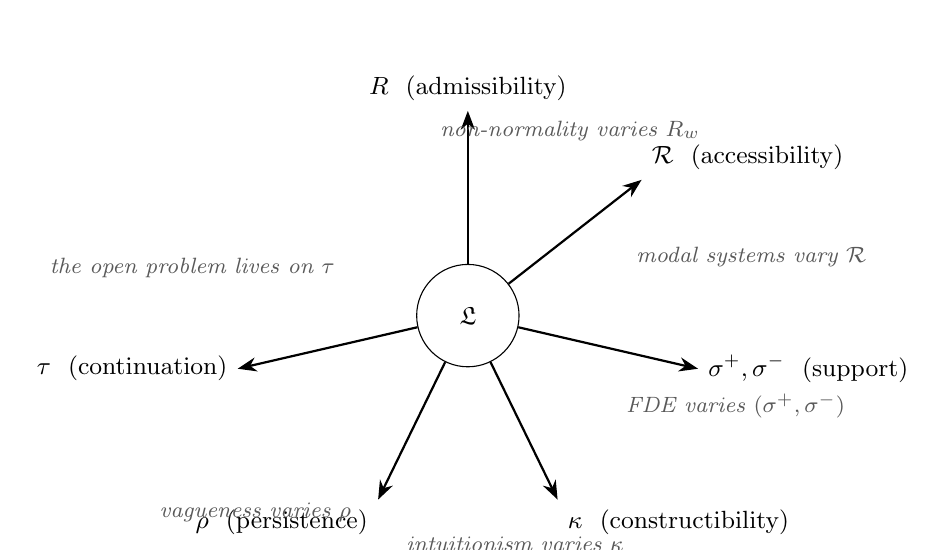
\begin{tikzpicture}[
  font=\small,
  ax/.style={-{Stealth[length=2.4mm]}, thick},
  coord/.style={font=\small},
  logic/.style={font=\footnotesize\itshape, gray!70!black}
]
\node[draw, circle, minimum size=13mm, inner sep=1pt] (L) at (0,0) {$\mathfrak{L}$};
\draw[ax] (L) -- (90:2.6)   node[coord, above] {$R$ \ (admissibility)};
\draw[ax] (L) -- (38:2.8)   node[coord, above right] {$\mathcal{R}$ \ (accessibility)};
\draw[ax] (L) -- (-13:3.0)  node[coord, right] {$\sigma^+, \sigma^-$ \ (support)};
\draw[ax] (L) -- (-64:2.6)  node[coord, below right] {$\kappa$ \ (constructibility)};
\draw[ax] (L) -- (-116:2.6) node[coord, below left] {$\rho$ \ (persistence)};
\draw[ax] (L) -- (-167:3.0) node[coord, left] {$\tau$ \ (continuation)};
\node[logic] at (1.3,2.35)  {non-normality varies $R_w$};
\node[logic] at (3.6,0.75)  {modal systems vary $\mathcal{R}$};
\node[logic] at (3.4,-1.15) {FDE varies $(\sigma^+,\sigma^-)$};
\node[logic] at (0.6,-2.9)  {intuitionism varies $\kappa$};
\node[logic] at (-2.7,-2.5) {vagueness varies $\rho$};
\node[logic] at (-3.5,0.6)  {the open problem lives on $\tau$};
\end{tikzpicture}
\caption{A schematic coordinate picture --- explicitly not a formal
definition --- of a logical regime
$\mathfrak{L} = (R, \mathcal{R}, \sigma^+, \sigma^-, \kappa, \rho, \tau)$
as a point in a space of independently variable structural dimensions.
The named non-classical logics do not sit along a single axis running
from classical to less classical; each alters a different coordinate,
which is this book's methodological thesis made visible. The tuple is a
mnemonic for the book's separations, not a definition the manuscript
supplies for every symbol.}
\label{fig:regime-coordinates}
\end{figure}

\hypertarget{the-open-problem-this-book-ends-on}{%
\section{The open problem this book ends on}\label{the-open-problem-this-book-ends-on}}

This is not a loose end awaiting a known fix. It's the point at which the
book's own framework ceases to close. The introduction's parameter arc
--- \(R \to (R,\mathcal{R}) \to (R,\mathcal{R},\sigma^+,\sigma^-) \to \text{local support/coherence} \to \text{repair and persistence} \to R_w\text{-dependent continuation}\) --- traced \(R\) progressively unpacking
into structure as each part of the book found the previous parameter
insufficient. Completing Parts II and V together shows what happens once
that unpacking reaches \(R\) itself: the thing Chapter 1 treated as fixed
background turns out, once identity across time is at stake, to be
capable of varying along the very trajectory it's supposed to govern.

\[x_t \xrightarrow{?} x_{t+1}, \qquad R_{x_t} \neq R_{x_{t+1}}.\]

Once admissibility is allowed to vary by state --- Chapter 7's \(R_w\),
needed to correctly place non-normal worlds --- trajectory-based identity
(Chapter 16) needs more than a sequence of admissible states connected by
\(\leadsto\). It needs an account of what makes a \emph{transition between
regimes} admissible, not merely what makes each endpoint admissible on
its own. Chapter 17's transition-object --- treating a transition as its
own kind of entity rather than a state satisfying an enriched valuation
--- is a candidate answer, floated at exactly the point in the book where
it became relevant and deliberately not promoted to a definition before
it had earned that status. Whether the right structure is a fixed choice
between \(R_{x_t}\) and \(R_{x_{t+1}}\), some combination of the two, or a
genuinely separate transition regime \(R_\gamma\), is left open. This
book's contribution is producing the question in a form precise enough
to be wrong about, not answering it --- and producing it as the place
where the framework's own regress of parameters runs out, rather than as
an item on a future-work list unconnected to everything before it.

\hypertarget{what-comes-next}{%
\section{What comes next}\label{what-comes-next}}

The correspondence ledger, not this conclusion, is the working document
for anyone extending this material --- it records status after drafting,
chapter by chapter, and should be checked before any claim in this
introduction or conclusion is relied upon for a further paper. Two
results look most likely to warrant standalone treatment ahead of the
full manuscript: the Mutual Non-Determination Proposition with its
realizability construction, and the \(R_w\)/continuation problem stated
above. Both are self-contained enough to be evaluated without the rest
of the book's apparatus, and both are the kind of result this project
was built to produce --- not agreement with Priest, and not a
redescription of him, but a specific, checkable place where this book's
own machinery says something Priest's framework alone does not.


\mainmatter

\part{I: Logic as Constraint}\label{part-i-logic-as-constraint}

\hypertarget{chapter-1-the-myth-of-a-single-logic}{%
\chapter*{Chapter 1 --- The Myth of a Single Logic}
\addcontentsline{toc}{chapter}{Chapter 1 --- The Myth of a Single Logic}
\markboth{Chapter 1 --- The Myth of a Single Logic}{Chapter 1 --- The Myth of a Single Logic}\label{chapter-1-the-myth-of-a-single-logic}}

The question this book opens with is not ``which logic is correct.'' It's:

\begin{quote}
What must remain invariant when representations are combined,
transported, refined, contradicted, or extended?
\end{quote}

That question doesn't presuppose an answer about how many truth values
there are, whether contradictions explode, or whether every proposition
is either true or false. It only presupposes that representations get
combined, moved, refined, sometimes contradicted, and sometimes extended
--- and asks what survives those operations. Logic, on this view, is the
study of what a given regime of transformation preserves.

\textbf{Consequence as preservation under admissible transformation.} Let a
\emph{state} be whatever a representational system currently commits to --- a
set of accepted propositions, a configuration of evidence, a model. Write
\(x \leadsto_R y\) for ``state \(y\) is reachable from state \(x\) under the
transformations a regime \(R\) permits.'' Logical consequence, in this
vocabulary, is:
\[\Gamma \models_R \varphi \quad\text{iff}\quad \text{every } R\text{-admissible extension of a state satisfying } \Gamma \text{ also satisfies } \varphi.\]
This is not a new definition invented to be exotic. It's the same shape
as the ordinary one --- consequence as truth-preservation across models ---
with one change: which transformations count as admissible is now a
parameter, \(R\), rather than fixed in advance.

\textbf{Classical logic is a point, not the origin.} Classical consequence is
what you get when \(R\) is set to its most stringent possible value: no
tolerance for a proposition and its negation both holding (no gluts), no
tolerance for a proposition holding neither way (no gaps), and
unrestricted propagation --- once a contradiction is admitted anywhere, every
proposition becomes admissible everywhere. That last clause is
\emph{ex falso quodlibet}, and it is worth noticing that it is a substantive
commitment about \(R\), not a logical necessity. Setting \(R\) to be less
strict --- tolerating gluts, tolerating gaps, restricting how far a local
failure propagates --- doesn't produce a rival to classical logic in the
sense of a competing claim about the same subject matter. It produces a
different regime, and classical logic is the member of that family
where the dial is turned to maximum strictness in every direction at
once. Later chapters (starting in Chapter 3, and given full formal
treatment in Part VI) will make this literal: the space of possible
regimes is a real object, not a metaphor, and classical logic is a
identifiable, describable point within it --- not the space's center, and
not its default.

\textbf{What this buys, and what it doesn't yet.} Reframing consequence this
way doesn't resolve any dispute about which logic to use for a given
purpose. What it does is stop the question from being framed as ``classical
logic, plus some deviant alternatives'' --- a framing that makes every
non-classical system look like a patch or a concession. If classical
logic is one regime among many, non-classical systems aren't deviations
requiring justification; they're other points that need locating, the
same way classical logic does. That relocation is this book's actual
project, and it starts, in the next chapter, from further back than
truth values themselves.

\hypertarget{chapter-2-distinction-before-truth}{%
\chapter*{Chapter 2 --- Distinction Before Truth}
\addcontentsline{toc}{chapter}{Chapter 2 --- Distinction Before Truth}
\markboth{Chapter 2 --- Distinction Before Truth}{Chapter 2 --- Distinction Before Truth}\label{chapter-2-distinction-before-truth}}

The ordinary starting point for logic takes truth values as given:
propositions are things that are true or false (or, in richer systems,
some fixed number of other things), and logic studies how those values
combine. This chapter argues that starting point already presupposes
something that itself needs an account --- and that the account, once
given, changes what a truth value turns out to be.

\textbf{The primitive act is distinction, not valuation.} Before anything can
be true or false, something has to be \emph{distinguished} --- carved out as a
determinate content that a truth value could even apply to. Asking
whether \(p\) is true already presupposes that \(p\) names a specific
distinction: this, as opposed to not-this, within some domain. That
prior act --- drawing the distinction --- is not itself a truth-evaluable
event. It's what makes truth-evaluation possible afterward.

\textbf{What follows from taking this seriously.} If distinction comes first,
a proposition's truth value shouldn't be treated as a primitive label
attached to it from outside. It should be \emph{read off} whatever process
generated the distinction and gathered evidence bearing on it. This is
not a promissory note for later --- it's exactly what Part VI does, in full
formal detail: Chapter 19 reconstructs the four Belnap-Dunn values not as
a stipulated alphabet but as the four possible outcomes of asking two
independent questions --- is there evidence \emph{for} this distinction holding,
and is there evidence \emph{against} it --- with \(N\), \(T\), \(F\), \(B\) arising as a
consequence of the support data rather than as an assumed starting
vocabulary. A glut isn't a fifth, exotic truth value bolted onto a
two-valued base; it's simply what ``both kinds of evidence present''
already means once truth values are treated as outputs rather than
inputs.

\textbf{Why this matters for the rest of the book.} Every non-classical system
covered in this book --- paraconsistent, intuitionistic, many-valued,
relevant, fuzzy --- is usually introduced by first fixing a set of truth
values and then giving rules for how they combine. That's a defensible
way to present a formal system, but it obscures a question worth asking
first: \emph{why these values, and not others?} Once truth values are treated
as consequences of a prior act of evidence-gathering over a distinction,
that question has an answer that doesn't have to be stipulated separately
for every logic in turn --- the values on offer are exactly the values a
given evidential structure can produce, and different logics turn out to
differ in what evidential structure they're built to track, not in an
arbitrary choice of alphabet.

\hypertarget{chapter-3-consistency-and-closure}{%
\chapter*{Chapter 3 --- Consistency and Closure}
\addcontentsline{toc}{chapter}{Chapter 3 --- Consistency and Closure}
\markboth{Chapter 3 --- Consistency and Closure}{Chapter 3 --- Consistency and Closure}\label{chapter-3-consistency-and-closure}}

``Consistent'' is usually treated as a single property a system either has
or lacks. This chapter argues that collapsing several genuinely different
notions into one word is a large part of why paraconsistency looks
paradoxical from the outside, and separates out the notions that actually
do the work.

\textbf{Local consistency.} A single region of a representational system ---
one patch, one context, one moment --- is locally consistent with respect
to a proposition \(p\) if it doesn't itself hold both \(p\) and its negation.
This is a property of one piece of the system in isolation, and nothing
about it says anything yet about how that piece relates to any other.

\textbf{Global consistency.} The whole system, taken together, is globally
consistent if no proposition is jointly supported and refuted once every
region's contributions are combined. This is a strictly different claim
from local consistency at every region individually --- a system can be
locally consistent everywhere and still fail to be globally consistent,
if different regions individually support and refute the same
proposition without either one containing a contradiction on its own.
(Part VI works this distinction out in full: Chapter 21's Glut-Free
Reconstruction Obstruction is precisely the condition under which local
data of this kind admits a globally consistent reading at all.)

\textbf{Constraint closure.} A regime \(R\) (Chapter 1's admissibility relation)
is closed under a class of transformations if performing them never
takes an admissible state outside admissibility. This is what actually
governs whether a local failure spreads: classical explosion is the
claim that \(R\) is closed under ``infer anything from a contradiction'' ---
which is one specific, and maximally permissive, choice of what counts
as an admissible move once a contradiction is present. Restricting
closure --- refusing to admit that move --- is not refusing to reason. It's
choosing a different, more conservative, and equally coherent notion of
what a contradiction is permitted to license.

\textbf{Representational coherence.} Separate again from all three above:
whether the pieces contributing to a proposition's support actually
\emph{agree} with each other, not merely whether they license the same
verdict. Two regions can both support \(p\) being true without their
support being the same support --- Chapter 20's coherence defect gives this
its formal treatment, and it is a genuinely fourth notion, not a
restatement of the first three. A system can be locally consistent
everywhere, globally consistent, closed under a conservative propagation
rule, and still be incoherent in this sense: agreeing on verdicts for the
wrong reasons.

Keeping these four separate --- local consistency, global consistency,
closure, coherence --- is not pedantry. Confusing any two of them is
exactly what makes claims like ``tolerating contradiction is dangerous''
sound like a single, self-evident worry, when in fact the danger (if
there is one) lives specifically in unrestricted closure, and neither
tolerating local gluts nor tolerating global disagreement nor tolerating
incoherent-but-agreeing witnesses is the same danger, or necessarily a
danger at all.

\hypertarget{chapter-4-failure-without-collapse}{%
\chapter*{Chapter 4 --- Failure Without Collapse}
\addcontentsline{toc}{chapter}{Chapter 4 --- Failure Without Collapse}
\markboth{Chapter 4 --- Failure Without Collapse}{Chapter 4 --- Failure Without Collapse}\label{chapter-4-failure-without-collapse}}

This chapter's title is meant as a thesis, not a description: a
representational system can fail --- locally, even repeatedly --- without
that failure collapsing the system into uselessness. What follows is an
account of the three different things ``failure'' can mean, and the
condition that actually separates recoverable failure from catastrophic
failure.

\textbf{Three modes of failure.}

\emph{Contradiction} is a local matter: a proposition and its negation both
supported, somewhere. On its own, per Chapter 3, this says nothing about
the health of the system as a whole.

\emph{Obstruction} is a structural matter, not a semantic one: local pieces of
evidence that individually make sense fail to assemble into a coherent
global picture, whether or not any single piece is itself contradictory.
Chapter 20's coherence defect is the formal name for this; it can occur
with no contradiction present at all.

\emph{Refusal} is neither of the above --- it's a deliberate constitutive act,
the decision that some transformation is not admissible, made in advance
rather than discovered as a failure after the fact. A regime that refuses
a move isn't failing to reason its way past a contradiction; it's
declining, as a matter of what the regime \emph{is}, to treat that move as
available.

\textbf{The distinction that actually matters: inconsistency versus
triviality.} Classical logic's core commitment is that these three modes
of failure, whenever they occur, must be treated identically --- as
signals that something has gone wrong that licenses anything at all to
follow. That identification is the actual source of explosion, and it's
worth stating as its own claim, separable from the rest of classical
logic's machinery: \emph{inconsistency} (a contradiction is present somewhere)
is not the same fact as \emph{triviality} (literally everything is now
derivable). A system can be inconsistent --- even irreducibly, permanently
inconsistent at some point --- without being trivial, provided its closure
conditions (Chapter 3) don't license the move from one to the other.
Priest's paraconsistent logics~\cite{priest2006} are, in this vocabulary, exactly regimes
where that licensing move has been withheld: contradiction is admitted as
a fact a system can contain, while triviality remains exactly as
catastrophic and exactly as avoidable as it always was.

\textbf{What ``failure without collapse'' actually requires.} Not tolerance for
error, and not a weakened notion of truth. It requires a regime whose
closure conditions don't route every local failure into global
collapse --- which is a structural property of \(R\), specifiable and
checkable, not a permissive attitude adopted toward contradiction for its
own sake. Part VI gives this requirement its sharpest form: Chapter 22's
repair machinery treats a glut as something with a repair cost, not as an
alarm demanding total system reset, and Chapter 21's separation of
contradiction from obstruction is precisely the demonstration that
``something has failed'' is not one fact but several, each with its own,
independently manageable consequences.

\hypertarget{status-of-this-draft}{%
\section{Status of this draft}\label{status-of-this-draft}}

Part I is written to be readable on its own --- a reader encountering only
these four chapters gets a complete philosophical case for treating
admissibility, distinction, and constrained closure as prior to truth
values and classical consistency --- while forward-referencing Part VI
honestly rather than pretending its formal results belong here. Nothing
in this draft is a new technical claim; the technical content is Part
VI's, established in Chapters 19--22. What's new here is the exposition:
stating the philosophical case in a form that motivates Part VI's
machinery before the reader has seen it, rather than only in retrospect.
One thing to watch when Parts II--V are drafted: Chapter 3's four-way
consistency/closure/coherence distinction is doing real setup work for
Part II's treatment of non-normal and impossible worlds, and Part V's
identity-under-transport material will likely want to lean on Chapter
2's distinction-before-truth framing rather than restate it --- worth
checking those connections hold once those parts exist, rather than
assuming they will.

\part{II: Worlds and Admissibility}\label{part-ii-worlds-and-admissibility}

\hypertarget{chapter-5-possible-worlds-as-admissible-states}{%
\chapter*{Chapter 5 --- Possible Worlds as Admissible States}
\addcontentsline{toc}{chapter}{Chapter 5 --- Possible Worlds as Admissible States}
\markboth{Chapter 5 --- Possible Worlds as Admissible States}{Chapter 5 --- Possible Worlds as Admissible States}\label{chapter-5-possible-worlds-as-admissible-states}}

Take the most conservative starting point available: a \textbf{world} \(w\) is a
state satisfying some governing regime \(R\) (Chapter 1) ---
\(w \in \operatorname{Adm}(R)\). As a first approximation, modal necessity
is invariance across the admissible states \(R\) reaches:
\[\Box_R p \quad\text{iff}\quad p \text{ holds throughout the } R\text{-accessible admissible states}.\]

This formula is provisional, and it's worth being honest about why
before using it for anything: it makes a single relation, \(R\), do two
jobs at once --- deciding which states are \emph{admissible at all}, and
deciding which admissible states are \emph{relevant to evaluating \(\Box\) at a
given world}. Those are not obviously the same question. Whether a state
satisfies the constraints governing the domain (admissibility) and
whether that state is one this particular world can ``see'' for purposes
of modal evaluation (accessibility) are different facts about a state,
and a definition that quietly identifies them is buying convenience at
the cost of a real distinction. Chapter 6 exists specifically to undo
that conflation; this chapter's job is only to introduce
\(\operatorname{Adm}(R)\) itself; readers should treat the box formula
above as scaffolding to be dismantled, not as this chapter's finished
result.

\textbf{What admissibility does and doesn't settle.} \(\operatorname{Adm}(R)\)
gives worlds a structural role --- the space of states a regime permits ---
without committing to what worlds metaphysically \emph{are}. Priest's own
survey of realism, actualism, and Meinongian approaches to possible
worlds is a debate about the second question; this framework only needs
an answer to the first one to get started, and Priest introduces
possible-world semantics~\cite{priest2008} in exactly this same methodologically modest
role before taking up the ontological question separately. Nothing here
forces a choice between treating admissible states as concretely existing
alternatives, as actualized constructions, or as objects that need not
exist in the same sense actual things do. The chapter deliberately leaves
that choice open, because nothing built so far depends on it being made.

\hypertarget{chapter-6-necessity-accessibility-and-invariance}{%
\chapter*{Chapter 6 --- Necessity, Accessibility, and Invariance}
\addcontentsline{toc}{chapter}{Chapter 6 --- Necessity, Accessibility, and Invariance}
\markboth{Chapter 6 --- Necessity, Accessibility, and Invariance}{Chapter 6 --- Necessity, Accessibility, and Invariance}\label{chapter-6-necessity-accessibility-and-invariance}}

Chapter 5's box formula conflated two relations. This chapter separates
them and, in doing so, corrects something the book's own outline had
gotten slightly wrong: ``necessity as invariance,'' stated without further
qualification, describes something looser than what Kripke semantics~\cite{kripke1963}
actually is. Kripke necessity is not invariance across admissible states
generally --- it's truth throughout the states a specific accessibility
relation selects, and that relation is additional structure, not a
byproduct of admissibility itself.

\textbf{Two parameters.} Let \(R\) continue to determine admissibility --- which
states satisfy the governing regime --- and introduce \(\mathcal{R}\),
independently, as the modal accessibility relation: \(w\mathcal{R}v\) means
\(v\) is relevant to evaluating modal claims at \(w\). Necessity becomes
\[w \models \Box p \quad\iff\quad \forall v\, (w \mathcal{R} v \Rightarrow v \models p),\]
with no requirement that \(\mathcal{R}\) be derived from, or even
compatible with, \(R\) in any fixed way. A state can be \(\mathcal{R}\)-related
to \(w\) without being \(R\)-admissible in the same sense \(w\) is (worlds
under consideration for modal purposes need not all satisfy identical
constraints), and a state can be \(R\)-admissible without being
\(\mathcal{R}\)-accessible from any world in particular (an admissible
state simply not under consideration from a given vantage point).

\begin{figure}[htbp]
\centering
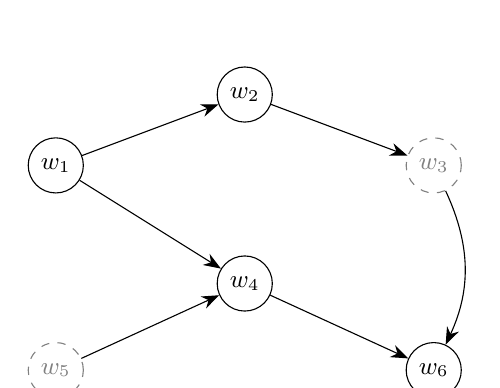
\begin{tikzpicture}[
  font=\small,
  adm/.style={draw, circle, minimum size=7mm, inner sep=0pt},
  inadm/.style={draw, circle, dashed, gray, minimum size=7mm, inner sep=0pt},
  acc/.style={-{Stealth[length=2.2mm]}}
]
\node[adm]   (w1) at (0,0)      {$w_1$};
\node[adm]   (w2) at (2.4,0.9)  {$w_2$};
\node[inadm] (w3) at (4.8,0)    {$w_3$};
\node[adm]   (w4) at (2.4,-1.5) {$w_4$};
\node[inadm] (w5) at (0,-2.6)   {$w_5$};
\node[adm]   (w6) at (4.8,-2.6) {$w_6$};
\draw[acc] (w1) -- (w2);
\draw[acc] (w2) -- (w3);
\draw[acc] (w1) -- (w4);
\draw[acc] (w4) -- (w6);
\draw[acc] (w5) -- (w4);
\draw[acc] (w3) to[bend left=25] (w6);
\end{tikzpicture}
\caption{Admissibility and accessibility are predicates of different
types. Arrows are accessibility edges $w \mathcal{R} v$; solid nodes are
$R$-admissible states, dashed gray nodes are not. $w_2 \mathcal{R} w_3$
holds even though $w_3 \notin \operatorname{Adm}(R)$ --- an accessible
world need not be admissible --- while $w_6 \in \operatorname{Adm}(R)$ is
reached only from an inadmissible state and from $w_4$; admissibility
generates no accessibility edge of its own. The rejected single-$R$
formulation of Chapter 5 would have made this frame inexpressible.}
\label{fig:adm-vs-acc}
\end{figure}

\textbf{What this buys.} Priest's various normal modal systems --- the
differences between K, T, S4, S5 and the rest --- are differences in what
structural properties \(\mathcal{R}\) is required to have: reflexivity,
transitivity, symmetry, and combinations of these, imposed on
accessibility specifically. None of this needs to touch \(R\) at all. A
system can strengthen or weaken its accessibility structure while
leaving admissibility exactly as it was, or vice versa --- change what
counts as an admissible state without touching which admissible states
are mutually accessible. Treating ``changing the modal logic'' and
``changing the admissibility regime'' as the same kind of move would have
been a real error, not a harmless simplification, and separating them
here is what makes the next chapter's argument possible at all.

\hypertarget{chapter-7-non-normal-and-impossible-worlds}{%
\chapter*{Chapter 7 --- Non-Normal and Impossible Worlds}
\addcontentsline{toc}{chapter}{Chapter 7 --- Non-Normal and Impossible Worlds}
\markboth{Chapter 7 --- Non-Normal and Impossible Worlds}{Chapter 7 --- Non-Normal and Impossible Worlds}\label{chapter-7-non-normal-and-impossible-worlds}}

This chapter is Part II's centerpiece, and it starts by retracting a
claim rather than building on one. An earlier working note in this
project's correspondence matrix rated ``a non-normal world deletes the
inference rule itself from what's admissible'' as a direct match to this
book's refusal machinery. That rating is downgraded here, from Direct to
Bridge, until this chapter actually establishes it --- asserting a
correspondence because the vocabulary sounds compatible is exactly the
kind of move this book has tried not to make, and there's no reason to
exempt this claim from that discipline.

\textbf{What Priest's non-normal worlds actually do, reconstructed first.} At
an ordinary (``normal'') world, \(\Box p\) is evaluated compositionally: true
iff \(p\) holds at every \(\mathcal{R}\)-accessible world, per Chapter 6. At
a \textbf{non-normal} world, that compositional rule is suspended --- the truth
value of \(\Box p\) at a non-normal world is not computed from what holds
at accessible worlds at all; it can be assigned independently, including
being false at a non-normal world even for a \(p\) that is a logical truth
holding at every other world. The consequence that matters most: modus
ponens itself, ordinarily a validity-preserving step everywhere, need
not hold at a non-normal world, because the world's evaluation behavior
is no longer tied to the mechanism that made modus ponens valid
elsewhere. \textbf{Impossible worlds} generalize this further still: worlds at
which the ordinary logical laws governing the rest of the framework may
simply fail to apply, not merely modal ones.

\textbf{What actually reproduces this, once reconstructed.} The behavior
above is not a targeted decision to decline one specific transformation
--- that would be refusal, in Chapter 4's sense, and refusal is a
\emph{Level 3} operation: a constitutive choice about which repair moves an
agent or system will make. What non-normal worlds do is different in
kind: the \emph{evaluation rule itself} is locally not in force. In this
book's vocabulary, that is best captured not by refusal but by treating
the regime as state-indexed rather than global: \(R_w\), a regime that can
itself vary from state to state, rather than one fixed \(R\) applied
everywhere with exceptions carved out afterward. A non-normal world is a
state whose local \(R_w\) simply does not include the closure condition
(Chapter 3) that would make \(\Box\)'s compositional rule, or modus ponens,
admissible moves there. This is a real correspondence, but a different
and more specific one than the original matrix entry claimed --- and it's
one this chapter has now actually earned, rather than assumed.

\textbf{The control case Part III supplies.} Before Part III existed, it
would have been tempting to treat ``impossible'' and ``contains a
contradiction'' as roughly the same idea. Part III makes that identification
untenable. An FDE world can contain both \(p\) and \(\neg p\) --- a glut, in
Chapter 10's sense --- while its consequence behavior remains perfectly
well-defined: Chapter 11's restricted propagation tells you exactly what
follows from that glut and what doesn't, compositionally, with no
suspension of any evaluation rule anywhere. Such a world is inconsistent
without being impossible in the sense this chapter has just defined, and
without being non-normal --- nothing about its evaluation machinery has
been switched off. Conversely, a non-normal or impossible state can fail
to validate modus ponens, or fail to respect \(\Box\)'s compositional rule,
while containing no glut at all --- every atomic proposition perfectly
determinate, no overdetermination anywhere, and still a state where some
structural rule simply isn't in force. These are three independent axes,
not one phenomenon under three names:

\[\boxed{\text{inconsistency} \neq \text{impossibility} \neq \text{non-normality}}\]

This belongs beside Chapter 3's four-way consistency/closure/coherence
split as the same kind of discipline applied to modal vocabulary instead
of evidential vocabulary. And it produces one sentence worth treating as
foundational for the rest of this book's modal material:

\begin{quote}
\textbf{Impossibility is indexed to a constraint regime; contradiction is
indexed to support.}
\end{quote}

A state is impossible or not relative to which \(R_w\) it's being measured
against --- the same state can be admissible under one regime and
inadmissible under a stricter one, with nothing about its content having
changed. A proposition is contradictory or not as a fact about its
support, full stop, independent of any regime. Confusing these two
coordinates --- treating the presence of a glut as automatically making a
world impossible --- would undo exactly the distinction Part III spent
four chapters establishing.

\hypertarget{chapter-8-conditionals-as-constrained-transport}{%
\chapter*{Chapter 8 --- Conditionals as Constrained Transport}
\addcontentsline{toc}{chapter}{Chapter 8 --- Conditionals as Constrained Transport}
\markboth{Chapter 8 --- Conditionals as Constrained Transport}{Chapter 8 --- Conditionals as Constrained Transport}\label{chapter-8-conditionals-as-constrained-transport}}

This chapter combines what earlier planning had kept as two separate
chapters --- strict implication and Lewis-style conditional logic~\cite{lewis1973} --- because
both are attempts at the same underlying question, and treating them
separately obscured that.

\textbf{The question.} Given a state \(w\) and a supposition \(p\) --- not
necessarily true at \(w\) --- which transformations away from \(w\) are
licensed when evaluating a further claim \(q\) under that supposition?
Strict implication answers this with maximum severity: \(p\) strictly
implies \(q\) iff \(q\) holds at every state where \(p\) holds, full stop,
which is exactly the source of strict implication's well-known paradoxes
(a necessary truth is strictly implied by anything, an impossible
proposition strictly implies anything) --- the same over-permissive
propagation problem Chapter 3 and Chapter 11 have already diagnosed in
other settings, showing up again here in conditional form. Lewis and
Stalnaker's similarity-sphere semantics answers it with an ordering:
evaluate \(q\) at the \(p\)-worlds \emph{most similar} to \(w\), rather than at all
of them.

\textbf{A candidate reformulation.} In this book's vocabulary, the question
becomes: given \(w\) and \(p\), which \(p\)-satisfying transformations of \(w\)
are \(R\)-admissible? Write this as
\[p \Rightarrow_R q\]
with truth depending on admissible \(p\)-transformations of \(w\) rather than
on material implication or on an externally supplied similarity metric.
This reformulation has real content --- it ties the conditional's behavior
to the same admissibility apparatus governing everything else in this
book, rather than treating conditionals as needing their own separate
primitive machinery --- but it should not be oversold. What it does not
yet do is tell you \emph{which} transformations count as admissible for a
given supposition, which is exactly the work Lewis's similarity ordering
was doing, and which this book's distinguishability geometry has been
suggested, elsewhere, as a candidate replacement for.

\textbf{The debt this chapter leaves open, deliberately.} It would be
premature to claim distinguishability geometry \emph{replaces} Lewisian
similarity spheres --- the correspondence matrix marks that Bridge, and
this chapter doesn't upgrade it, because nothing here has shown the
similarity ordering can actually be derived rather than separately
stipulated. The honest question to end on: can a similarity ordering
over \(p\)-satisfying transformations be derived from the geometry of
admissible transformation itself --- from the same structure that already
determines \(\operatorname{Adm}(R)\) and \(R_w\) --- rather than supplied as
independent primitive structure the way Lewis's own semantics requires?
If yes, conditionals stop needing a bespoke ordering relation and become
a further consequence of admissibility geometry already on hand. If no,
conditionals are a genuinely independent piece of structure this
framework hasn't reduced, and the book should say so plainly rather than
paper over it. This chapter poses that question; it does not answer it.

\hypertarget{status-of-this-draft}{%
\section{Status of this draft}\label{status-of-this-draft}}

Part II's progression --- alternative states, accessibility, violations of
admissibility, transport under supposition --- holds together, and the
chapter that mattered most going in, Chapter 7, survived contact with
Part III's control case rather than needing to be softened to fit it.
One real result came out of testing rather than assuming: the original
correspondence-matrix claim about non-normal worlds and refusal was
wrong in its specifics, even though something in that neighborhood is
true --- the corrected version (state-indexed regime \(R_w\), not refusal)
is more precise and, on inspection, more defensible than the claim it
replaced. Chapter 8 ends with a named open debt rather than a premature
claim, per instruction. Worth checking once Part V is drafted: Chapter 7's
\(R_w\) move (regimes varying by state) is very close to what Part V's
identity-under-transport material will need for tracking a single
entity across states with potentially different local constraints ---
that connection wasn't planned in advance and should be verified rather
than assumed to hold.

\part{III: Gaps, Gluts, and Propagation}\label{part-iii-gaps-gluts-and-propagation}

\hypertarget{chapter-9-gaps-determination-without-bivalence}{%
\chapter*{Chapter 9 --- Gaps: Determination Without Bivalence}
\addcontentsline{toc}{chapter}{Chapter 9 --- Gaps: Determination Without Bivalence}
\markboth{Chapter 9 --- Gaps: Determination Without Bivalence}{Chapter 9 --- Gaps: Determination Without Bivalence}\label{chapter-9-gaps-determination-without-bivalence}}

Chapter 2 argued that distinction precedes truth: before a proposition
can be true or false, something has to be carved out as a determinate
content for a truth value to apply to. This chapter takes the next step,
and it's a smaller one than it might look: once truth values are read off
evidence rather than assumed in advance, the possibility that evidence is
simply \emph{absent} has to be taken seriously as its own case, not folded
into ``false'' or treated as a defect.

\textbf{Two independent questions, minimally.} Ask, of a proposition \(p\): is
there positive support for \(p\) --- evidence, a witness, a derivation, in
whatever sense support is available in the context at hand? And,
separately: is there negative support for \(p\)? Nothing forces these two
questions to have correlated answers. A failure to find positive support
does not, by itself, hand you negative support --- the absence of a reason
to affirm something is not a reason to deny it. That's not a special
principle needing independent defense; it's simply what it means for the
two questions to be genuinely two questions rather than one question
asked twice.

\textbf{What underdetermination is, and isn't.} When neither kind of support
is present, call \(p\) \textbf{underdetermined} at that context. This is not a
third truth value smuggled in alongside true and false --- it's what ``no
answer to either question yet'' already amounts to, once the two
questions have been separated. Priest's own examples fit cleanly here
without needing modification: a definite description with no referent
(``the current King of France is bald'') supplies neither positive nor
negative support for predications about its subject, because there's no
subject there to support anything about. A future contingent --- a claim
about tomorrow's sea battle, asked today --- has no positive support (the
battle hasn't happened) and, importantly, no negative support either (its
non-occurrence hasn't happened yet), which is a different situation from
a claim that has been actively falsified.

\textbf{Why a gap is not an obstruction.} This is the point worth stating
carefully, because it will matter again once Part VI generalizes this
material: underdetermination is harmless in a specific, checkable sense.
An underdetermined proposition imposes no obstacle to reconstructing a
larger picture around it --- you can always extend an underdetermined case
with more information later, in either direction, without having to
retract anything you'd previously committed to, because you hadn't
committed to anything yet. A gap doesn't need repairing; it needs
filling in, which is a different operation with a different cost. That
distinction --- between a state that costs nothing to extend and a state
that actively resists coherent extension --- is what separates this
chapter from the next one, and conflating them is the single most common
way nonclassical semantics gets misread as a uniform tolerance for
``weirdness,'' when in fact gaps and gluts are opposite kinds of case, not
two flavors of the same thing.

\hypertarget{chapter-10-gluts-contradiction-as-retained-information}{%
\chapter*{Chapter 10 --- Gluts: Contradiction as Retained Information}
\addcontentsline{toc}{chapter}{Chapter 10 --- Gluts: Contradiction as Retained Information}
\markboth{Chapter 10 --- Gluts: Contradiction as Retained Information}{Chapter 10 --- Gluts: Contradiction as Retained Information}\label{chapter-10-gluts-contradiction-as-retained-information}}

Chapter 9 established that absence of support in one direction doesn't
force support in the other. This chapter is about what happens when both
directions are actually supported at once --- and argues that the right
response is not automatically to treat this as an error state requiring
correction.

\textbf{The four statuses, from two coordinates.} With both positive and
negative support now genuinely in play, the same construction from
Chapter 9 yields four cases rather than two: no support either way
(underdetermined, Chapter 9's subject), positive support only, negative
support only, and --- the new case --- both. Call a proposition with both
positive and negative support \textbf{overdetermined}. This is Belnap and
Dunn's~\cite{belnap1977,dunn1976} fourth value, arrived at the same way the other three were: as a
consequence of what the support data actually contains, not as a
stipulated addition to a prior two-valued base.

\begin{figure}[htbp]
\centering
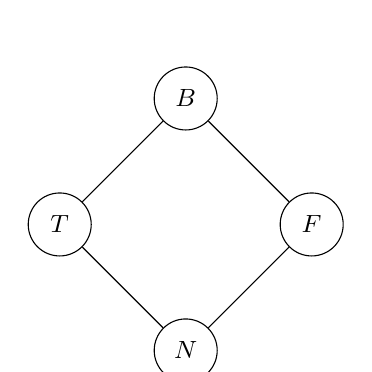
\begin{tikzpicture}[
  node distance=1.6cm and 1.6cm,
  val/.style={draw, circle, minimum size=8mm, inner sep=0pt, font=\small},
  lbl/.style={font=\footnotesize, midway, sloped}
]
\node[val] (B) at (0,1.6) {$B$};
\node[val] (T) at (-1.6,0) {$T$};
\node[val] (F) at (1.6,0) {$F$};
\node[val] (N) at (0,-1.6) {$N$};
\draw (N) -- (T);
\draw (N) -- (F);
\draw (T) -- (B);
\draw (F) -- (B);
\end{tikzpicture}
\caption{The Belnap--Dunn information lattice $\mathbb{F} = \{N,T,F,B\}$
under the information order $\sqsubseteq_k$. $N$ is bottom (no support),
$B$ is top (both polarities), and $T,F$ are incomparable. Consequently
$T \vee_k F = B$: pooling positive-only and negative-only support
produces a glut by construction, not by exception.}
\label{fig:belnap-lattice}
\end{figure}

\textbf{The claim that matters is stronger than ``some propositions are both
true and false.''} That phrasing makes overdetermination sound like a
metaphysical oddity --- a strange fact about certain propositions. The
sharper claim is procedural: contradictory evidence does not need to be
\emph{deleted} merely because it is contradictory. Given two conflicting
bodies of evidence, a system has a choice about what to do with the
conflict, and ``erase one side'' is only one option among several, not the
obviously correct one. Chapter 4's refusal machinery is exactly what
makes the alternative precise: a regime can \emph{refuse} the deletion ---
decline, as a constitutive matter, to treat ``these conflict'' as
sufficient grounds for discarding either witness --- and retain both. That
refusal is not indecision or error-tolerance. It's a principled
commitment to not letting a specific kind of local conflict force a loss
of information that nothing yet justifies losing.

\textbf{What this is not.} Overdetermination is not the same epistemic
situation as uncertainty. ``We don't know whether \(p\)'' is Chapter 9's
underdetermination --- absence of support in both directions.
``We have positive and negative support for \(p\)'' is a different fact
entirely --- presence of support in both directions --- and treating the two
as interchangeable (as ordinary language sometimes does, calling both
situations ``unclear'') erases a distinction the rest of this book depends
on. Priest's semantic paradoxes (the Liar sentence, under a sufficiently
expressive language, genuinely supports both its own truth and its own
falsity by the ordinary rules governing truth predicates), and the
existence of legal and normative systems that contain live, unresolved
contradictions without therefore becoming useless, are both cases of
overdetermination in this sense, not cases of not-yet-knowing.

\textbf{The asymmetry, stated once, philosophically, ahead of its formal
treatment.} Chapter 9's gaps and this chapter's gluts are not mirror
images of each other, whatever the symmetry of the four-value notation
suggests. A gap costs nothing and obstructs nothing; it is the default,
harmless case. A glut is the substantive case --- the one that actually
requires the rest of this book's machinery to handle responsibly. Part
VI gives this asymmetry an exact formal statement; here it is enough to
notice that ``insufficient support'' and ``incompatible support'' are not
symmetric failures, and treating them as if they were is a mistake this
book avoids from the outset rather than discovering later.

\hypertarget{chapter-11-paraconsistency-why-contradiction-does-not-propagate}{%
\chapter*{Chapter 11 --- Paraconsistency: Why Contradiction Does Not Propagate}
\addcontentsline{toc}{chapter}{Chapter 11 --- Paraconsistency: Why Contradiction Does Not Propagate}
\markboth{Chapter 11 --- Paraconsistency: Why Contradiction Does Not Propagate}{Chapter 11 --- Paraconsistency: Why Contradiction Does Not Propagate}\label{chapter-11-paraconsistency-why-contradiction-does-not-propagate}}

Chapter 4 separated inconsistency from triviality and left one question
open: what has to be true of a system's propagation rules for the
former not to become the latter? This chapter answers it, and it is the
technical centerpiece of Part III.

\textbf{Explosion as one specific propagation rule, not a logical necessity.}
Classically, from \(p\) and \(\neg p\), anything follows --- most directly via
disjunctive syllogism: from \(p \vee q\) and \(\neg p\), infer \(q\); since \(p\)
is available, \(p \vee q\) holds for any \(q\) whatsoever, and \(\neg p\) is
also available, so \(q\) follows, for arbitrary \(q\). Every step in that
derivation is individually classically valid. The question this chapter
asks is not whether the derivation is classically valid --- it is --- but
whether a system is \emph{obligated} to make disjunctive syllogism available
at a point where both \(p\) and \(\neg p\) are independently supported.

\textbf{Why the answer can be no, without giving up inference generally.}
Consider a proposition \(p\) that is overdetermined --- both \(p\) and \(\neg p\)
supported, in Chapter 10's sense. Disjunctive syllogism, applied here,
uses the \emph{positive} support for \(p\) to license \(p \vee q\), and then uses
the \emph{negative} support for \(p\) (i.e., \(\neg p\)) to discharge the \(p\)
disjunct and leave \(q\) standing --- treating the negative support as if it
straightforwardly eliminated the positive support's contribution. But
that is exactly the move Chapter 10 argued a system need not make: the
negative support doesn't erase the positive support in an overdetermined
case, by definition --- that's what overdetermination \emph{is}. Disjunctive
syllogism's second step silently assumes the positive and negative
supports can't coexist, which is precisely false at an overdetermined
point. Blocking disjunctive syllogism at exactly these points is not an
ad hoc patch to avoid an unwanted conclusion; it's the direct consequence
of taking Chapter 10's retained-information picture seriously rather than
only in the abstract.

\textbf{The general propagation principle.} Stated once, for use throughout
the rest of the book: a local failure should propagate only as far as
the dependency structure connecting it to other propositions actually
warrants --- not automatically to every proposition in the language, which
is what unrestricted closure (Chapter 3) does by default. Restricting
propagation at exactly the step that assumes what an overdetermined
proposition specifically denies is what keeps a contradiction local. This
is also why paraconsistency is not ``logic with the brakes cut'' --- if
anything, it's the more conservative regime: it declines to license an
inferential step whose validity depended on an assumption (that positive
and negative support are mutually exclusive) that the very situation
under discussion has already falsified.

\hypertarget{chapter-12-repair-and-classical-recapture}{%
\chapter*{Chapter 12 --- Repair and Classical Recapture}
\addcontentsline{toc}{chapter}{Chapter 12 --- Repair and Classical Recapture}
\markboth{Chapter 12 --- Repair and Classical Recapture}{Chapter 12 --- Repair and Classical Recapture}\label{chapter-12-repair-and-classical-recapture}}

Part III closes by asking what a system should actually \emph{do} once it
has an overdetermined proposition on its hands, rather than merely
tolerating its presence.

\textbf{The merge.} Given several independent bodies of evidence
\(s_1, \dots, s_n\) bearing on \(p\) --- not yet organized spatially into
patches or a cover, simply distinct sources --- their combination is given
by the pointwise information merge
\[M(p) = \bigvee_i s_i(p),\]
the least assignment that retains everything each source individually
supplied. This always exists (no combination of sources can fail to have
a merge), and \(M(p)\) comes out overdetermined exactly when the sources
collectively supply both positive and negative support for \(p\) --- which
is precisely Chapter 10's notion, arrived at now as a consequence of
combining evidence rather than stipulated about a single source.

\textbf{Why the classical alternative genuinely fails, rather than merely
being undesirable.} Suppose a system insists on a glut-free
reconstruction --- a single, classical assignment of true-or-false to \(p\)
that's consistent with everything the sources supplied. If the sources
jointly supply both positive and negative support, no such assignment
exists: anything siding with the positive evidence contradicts the
negative evidence, and vice versa. This is a genuine non-existence
result, not a preference --- a classical, no-glut regime has \emph{no}
admissible reconstruction of that evidence at all. Paraconsistency's
contribution here is not ``tolerating an error the classical approach
would have caught.'' It's supplying a reconstruction --- \(M(p) = B\) --- where
the classical regime supplies none. The paraconsistent regime has
strictly more admissible outcomes available to it, and this is one of
them being used, not an error being excused.

\textbf{Classical recapture.} A system that admits overdetermination
everywhere it's forced to, but nowhere else, and actively minimizes how
much of the language ends up overdetermined, recovers classical behavior
almost everywhere while preserving exactly the local gluts the evidence
actually demands --- this is Priest's minimally inconsistent LP, and in
this book's vocabulary it is a repair operator biased toward
consistency: pay the cost of a glut only where the evidence leaves no
alternative, default to classical, glut-free assignment everywhere else.
This is the first appearance, at the level of a single proposition and
its sources, of a idea Part VI will generalize considerably: repair is
not the opposite of classical reasoning, it's classical reasoning with an
escape hatch for the specific cases where classical reasoning has
nowhere to go.

\textbf{The arc of Part III, and what it deliberately withholds.} Chapters
9--12 trace one continuous line: underdetermination, independent support,
overdetermination, restricted propagation, repair. Everything in this
arc is local and order-theoretic --- a fact about single propositions and
the evidence bearing on them, not about how evidence distributed across
many regions of a larger structure does or doesn't cohere with itself.
That second question --- what happens once these support objects are
localized over a genuine cover, and whether local overdetermination has
anything to do with whether the pieces of evidence agree with each other
in the first place --- is Part VI's question, not this one's, and this
part has deliberately not reached for it. Cohomology, coherence defects,
and the distinction between a glut and an obstruction to gluing are held
back on purpose: introducing them here would answer Part VI's question
before its own machinery exists to ask it properly, and would blur
exactly the local/global independence that turns out to be one of this
book's more original claims.

\hypertarget{status-of-this-draft}{%
\section{Status of this draft}\label{status-of-this-draft}}

Written to be self-contained: a reader who stops after Part III has a
complete, correct account of gaps, gluts, paraconsistency, and repair at
the level of individual propositions and their evidence, without needing
anything from Part VI. Deliberately withheld throughout: any mention of
covers, patches, coherence defects, or cohomology --- those are held for
Part VI specifically so that Part III's account doesn't accidentally
answer, or foreclose, the question of whether local nonclassical
valuation and global structural obstruction are related. One thing to
verify once Part VI is revised last (per the drafting order settled on):
that Chapter 12's merge proposition and Part VI's Chapter 21 restatement
of the same result are stated compatibly, since they're now the same
claim appearing at two different levels of generality and any drift
between the two would be worth catching before either is called final.

\part{IV: Construction, Vagueness, and Degree}\label{part-iv-construction-vagueness-and-degree}

\hypertarget{chapter-13-truth-as-construction}{%
\chapter*{Chapter 13 --- Truth as Construction}
\addcontentsline{toc}{chapter}{Chapter 13 --- Truth as Construction}
\markboth{Chapter 13 --- Truth as Construction}{Chapter 13 --- Truth as Construction}\label{chapter-13-truth-as-construction}}

Part III built truth values from independent positive and negative
support: a proposition is true when there's evidence for it, false when
there's evidence against, both or neither as the data allows. This
chapter asks a question that support alone doesn't answer, and it's
worth being precise about why the two are different before claiming any
correspondence between them.

\textbf{What support doesn't distinguish.} Positive support for \(p\), in
Part III's sense, is silent about \emph{how} that support was obtained. A
proof by contradiction --- assume \(\neg p\), derive an absurdity, conclude
\(p\) --- counts as positive support exactly as much as a direct construction
does; nothing in Chapters 9--12 cared about the difference. Intuitionism
cares about exactly this difference, and treats it as decisive rather
than incidental: on the BHK (Brouwer-Heyting-Kolmogorov)~\cite{heyting1956} reading, a proof
of \(p \to q\) is a specific procedure converting any proof of \(p\) into a
proof of \(q\); a proof of \(p \vee q\) is a proof of one disjunct together
with a specification of \emph{which} one; and a proof of \(p\) simply is a
witness --- something producible, not merely something whose existence
follows from the absurdity of its absence. Excluded middle, \(p \vee \neg p\), fails on this reading not because intuitionists doubt that every
proposition is either provable or refutable in some further sense, but
because \emph{having a proof of the disjunction} requires having a proof of
one side specifically, and there are propositions for which neither is
currently in hand.

\textbf{A genuinely separate axis, not a restriction of Part III's.} It would
be a mistake to read intuitionistic truth as ``Part III's positive support,
but stricter'' --- as though constructive proof were simply positive support
held to a higher standard along the same dimension. The two are asking
different questions. Part III asks whether evidence exists, for or
against, independent of its provenance. Intuitionism asks, given that
evidence exists, whether it takes the specific form of an exhibitable
construction --- and this question is orthogonal to the evidential
question, not a refinement of it. A piece of positive support could in
principle be a valid, non-constructive derivation (existence without
witness) or a genuine construction (existence with witness); Part III's
apparatus doesn't distinguish these, and didn't need to for the results
it was building.

\textbf{Proof as reconstruction path.} With that separation in place, the
correspondence this book has anticipated since its opening chapters can
be stated properly rather than merely gestured at: a constructive proof
of \(p\) is a \textbf{reconstruction path} to \(p\) in the sense this book's
reconstruction cluster already uses that phrase --- a specific, traceable
route by which \(p\) becomes available, as opposed to a bare guarantee that
some route exists. The precise place this shows up, rather than the
looser slogan it's tempting to reach for: intuitionistic logic does not
in general license
\[\neg\neg p \to p,\]
because a construction that transforms every attempted proof of \(\neg p\)
into an absurdity is not thereby a construction of \(p\) itself --- it shows
\(\neg p\) is unavailable, not that \(p\) is available, and those are
different accomplishments. That is structurally the same refusal this
book's repair machinery makes when it declines to treat ``no admissible
reconstruction currently known'' as equivalent to ``no admissible
reconstruction exists'': both positions insist that availability has to be
demonstrated by production, not inferred from the unavailability of its
negation. Stating the correspondence at the level of \(\neg\neg p \to p\)
specifically, rather than at the level of a general slogan about
``inferring existence from absurdity,'' is what keeps this correspondence
exact rather than approximate.

\textbf{What this now makes visible.} Between Part III and this chapter, the
book has quietly assembled three independent coordinates rather than
one: positive support, negative support, and constructibility. An
assertion can carry positive support without a constructive witness (a
valid non-constructive derivation); once a construction is available, it
supplies a particularly strong species of positive support, but the
converse doesn't hold. This isn't a result this chapter needs to develop
further yet --- it's simply worth naming, since it's early evidence for
this book's larger claim that nonclassical logics needn't be arranged
along one axis of ``how far from classical,'' but can differ along several
independent dimensions at once.

\hypertarget{chapter-14-degrees-of-distinction}{%
\chapter*{Chapter 14 --- Degrees of Distinction}
\addcontentsline{toc}{chapter}{Chapter 14 --- Degrees of Distinction}
\markboth{Chapter 14 --- Degrees of Distinction}{Chapter 14 --- Degrees of Distinction}\label{chapter-14-degrees-of-distinction}}

Kleene's and Łukasiewicz's~\cite{lukasiewicz1920} many-valued logics assign propositions values
along a chain --- three values, finitely many, or a continuum --- rather than
reading four values off two independent evidential coordinates the way
Part III did. This chapter's main work is resisting an easy but wrong
move: treating degree-valued logics as a generalization of FDE, with
Part III's four values as a coarse special case of a finer many-valued
scheme.

\textbf{Why the two shouldn't be collapsed.} FDE's four values arise from
asking two independent yes/no questions --- positive support, negative
support --- and reading off one of four combinations. Nothing about that
construction involves degree; \(T\) and \(B\) aren't more or less true than
each other, they're different combinations of a binary fact along two
axes. A many-valued logic, by contrast, is committed to propositions
admitting \emph{degrees} of truth along a single ordered scale --- not ``how much
evidence in which of two directions'' but ``how true, full stop,'' a
fundamentally different kind of quantity. Forcing these into one
framework --- treating Łukasiewicz values as refinements of FDE's four
points, say --- would blur a distinction Part III spent real effort
establishing: that gaps and gluts are about evidential structure, not
about a proposition occupying some intermediate position on a truth
continuum. Keep them as genuinely separate formal commitments, useful for
different purposes, rather than one subsuming the other.

\textbf{What degree actually tracks --- and what's this book's addition rather
than the logic's own content.} It would overclaim to say many-valued
semantics \emph{means} resolution-stability. A value like \(0.7\), on its own,
carries no built-in commitment to surviving 70\% of some refinement
process --- depending on the system, intermediate values play quite
different semantic roles (partial belief, verisimilitude, membership
degree), and none of Kleene's or Łukasiewicz's own machinery forces a
resolution-theoretic reading. What this chapter proposes is narrower and
should be labeled as an addition, not a discovery: \textbf{resolution-stability
is one interpretation of degree, proposed here to connect degree
semantics to this book's distinguishability geometry} --- not something
many-valued logic already meant on its own.

Stated with the structure this actually requires: fix a resolution
parameter \(\lambda \in \Lambda\) and let \(v_\lambda(p) \in [0,1]\) be the
degree assigned to \(p\) at resolution \(\lambda\). Two different objects
now need to be kept apart. \(v_\lambda(p)\) is a single number --- the degree
at one fixed resolution, no more informative than an ordinary many-valued
assignment. The \textbf{resolution profile}, \(\lambda \mapsto v_\lambda(p)\),
is a function tracking how that degree moves as resolution changes, and
it is \emph{only} the profile that carries the structure the next chapter
needs. Nothing about many-valued logic itself supplies a family
\(\{v_\lambda\}_{\lambda \in \Lambda}\) rather than one value --- that
family, and the profile built from it, is this chapter's proposed
addition, offered as a testable interpretation rather than presented as
inherent in the semantics it's applied to.

\hypertarget{chapter-15-boundary-cases}{%
\chapter*{Chapter 15 --- Boundary Cases}
\addcontentsline{toc}{chapter}{Chapter 15 --- Boundary Cases}
\markboth{Chapter 15 --- Boundary Cases}{Chapter 15 --- Boundary Cases}\label{chapter-15-boundary-cases}}

The sorites paradox --- remove one grain from a heap, and it's still a
heap; repeat enough times, and it isn't --- is usually treated as a puzzle
about vagueness specifically, calling for its own bespoke machinery
(supervaluation, degree-valued semantics, epistemicism about a sharp but
unknowable cutoff). This chapter argues it's an instance of something
this book already has a name for, once Chapter 14's reframing is taken
seriously.

\textbf{The concept that was promised earlier and now gets built.} Much
earlier in this project's development, a distinction surfaced between two
different ways local data can fail to support a coherent global picture:
\emph{compatibility obstruction} (Part III and Part VI's subject --- sections,
or bodies of evidence, disagreeing with each other) and a second,
distinct notion, noted at the time and deliberately not developed until
a chapter existed that actually needed it. That chapter is this one.

\textbf{Getting the definition right --- a first version breaks on contact with
transitivity.} The tempting statement is: every adjacent resolution
agrees exactly, and yet the extremes disagree. That doesn't work, and
it's worth seeing why before stating the correct version, since the
failure is instructive. If \(v_\lambda = v_{\lambda'}\) for every adjacent
pair in a chain of resolutions, transitivity of equality forces the two
endpoints to agree as well --- exact local agreement all the way down
\emph{cannot} produce global disagreement; something else in the structure
would have to be non-transitive, scale-dependent, or lossy for that to
happen, and ``exact agreement everywhere, yet disagreement overall'' is
simply not a coherent way to state what sorites-style predicates are
doing.

\textbf{Dispersion obstruction, stated correctly.} What actually happens is
not exact agreement failing to propagate --- it's \emph{small} variation
accumulating past a threshold. Suppose consecutive resolutions satisfy
\[d\big(v_{\lambda_i}, v_{\lambda_{i+1}}\big) \leq \epsilon_i\]
at every step, where each individual \(\epsilon_i\) falls beneath whatever
counts as a noticeable difference at that step --- but the \emph{sum}
\(\sum_i \epsilon_i\) need not be small at all. Every single transition can
be locally negligible while the accumulated trajectory crosses the
predicate's macroscopic boundary. This is genuinely different from
compatibility obstruction, not merely compatibility obstruction with a
scale parameter bolted on:

\begin{quote}
\textbf{Compatibility obstruction is failure to agree. Dispersion obstruction
is failure of locally small variation to remain globally small under
iteration.}
\end{quote}

\textbf{A toy example, to make the mechanism concrete.} Let \(v(n) = n/1000\)
for \(n\) grains removed. Each single removal changes the value by exactly
\(|v(n) - v(n-1)| = 0.001\) --- negligible by any reasonable local threshold.
Traversing the entire chain gives \(|v(1000) - v(0)| = 1\) --- the full
range. Nothing contradictory occurred at any step. Nothing failed to
agree at any overlap. Tiny changes simply accumulated, which is precisely
what a persistence functional needs to detect: \(\mathcal{P}[s] \to 0\)
under repeated coarsening should track accumulated small displacement,
not the presence or absence of any single disagreement.

\begin{figure}[htbp]
\centering
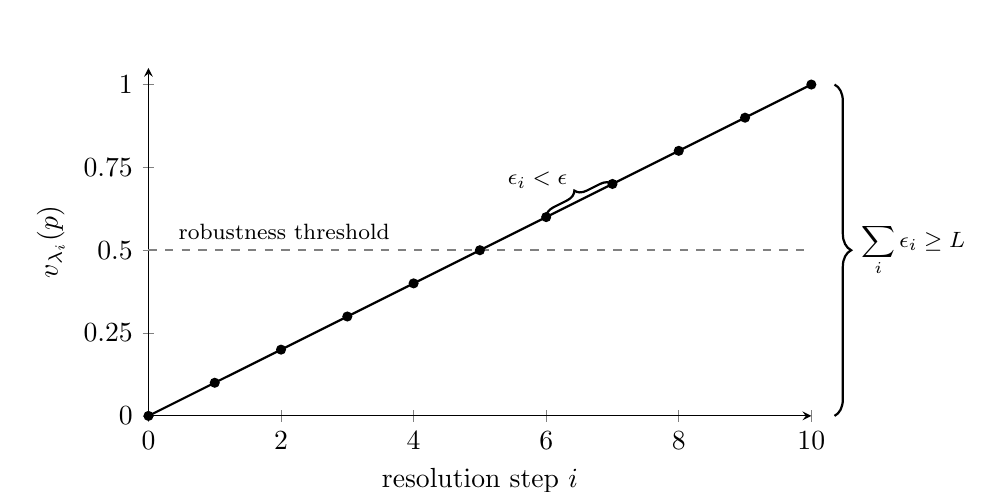
\begin{tikzpicture}
\begin{axis}[
  width=10cm, height=6cm,
  xlabel={resolution step $i$},
  ylabel={$v_{\lambda_i}(p)$},
  xmin=0, xmax=10, ymin=0, ymax=1.05,
  xtick={0,2,...,10},
  ytick={0,0.25,0.5,0.75,1},
  axis lines=left,
  every axis plot/.append style={black},
  clip=false
]
\addplot[mark=*, mark size=1.4pt, thick] coordinates {
(0,0) (1,0.1) (2,0.2) (3,0.3) (4,0.4) (5,0.5) (6,0.6) (7,0.7) (8,0.8) (9,0.9) (10,1.0)
};
\addplot[dashed, gray, thick, domain=0:10] {0.5}
  node[pos=0.03, above, black, font=\footnotesize, anchor=south west] {robustness threshold};
\draw[decorate, decoration={brace, amplitude=4pt}, thick]
  (axis cs:6,0.6) -- (axis cs:7,0.7)
  node[midway, above left=1pt, font=\footnotesize] {$\epsilon_i < \epsilon$};
\draw[decorate, decoration={brace, mirror, amplitude=6pt}, thick]
  (axis cs:10.35,0) -- (axis cs:10.35,1.0)
  node[midway, right=6pt, font=\footnotesize] {$\displaystyle\sum_i \epsilon_i \geq L$};
\end{axis}
\end{tikzpicture}
\caption{Dispersion under refinement. Each increment
$|v_{\lambda_{i+1}}(p) - v_{\lambda_i}(p)| = \epsilon_i$ falls below any
reasonable local threshold $\epsilon$, yet the accumulated displacement
$\sum_i \epsilon_i$ crosses the predicate's robustness threshold (dashed).
Local smallness does not imply global persistence. No step contains a
disagreement, so this failure is invisible to Chapter 21's overlap
comparison --- dispersion and compatibility obstruction are different
mechanisms.}
\label{fig:dispersion}
\end{figure}

\textbf{Why this had to wait for Chapter 14, and couldn't live in Part III or
Part VI.} Compatibility obstruction, as built in Part III and formalized
further in Part VI, is a fact about disagreement between fixed pieces of
local data at one resolution --- it has no notion of \emph{scale} built into it
at all; two patches either agree or they don't, full stop. Dispersion
obstruction needs a family of resolutions, a distance between values at
adjacent resolutions, and a way of accumulating that distance across the
whole family --- precisely the resolution-profile structure Chapter 14
introduced and Parts III and VI never needed, because bare agreement or
disagreement doesn't carry a magnitude the way accumulation requires.
Vagueness, on this account, isn't a fourth kind of nonclassical semantics
standing beside gaps, gluts, and constructive failure, and it also isn't
merely ``compatibility obstruction plus a scale parameter'' --- it's a
genuinely different mathematical mechanism, a third failure mode
distinguishable from the other two by what it actually requires to
detect it:

\[\boxed{\text{compatibility} \neq \text{continuity} \neq \text{persistence}}\]

Compatibility (Part III, Part VI) asks whether fixed local pieces agree.
Continuity, in whatever sense a topology on a space of configurations
might supply, asks which configurations count as \emph{nearby}. Persistence ---
this chapter's actual subject --- asks whether small displacement,
repeatedly accumulated, stays small. A bare topology encodes the second
without automatically supplying the third: nearness alone doesn't hand
you a magnitude of accumulated displacement unless something further
(a metric, a uniformity, a filtration, or the \(\mathcal{P}\) functional
used here) is layered on top of it.

\textbf{What this chapter leaves open.} Whether \(\mathcal{P}[s] \to 0\), defined
via accumulated pairwise distance, is the right formal target isn't
settled here --- the choice of persistence functional is a modeling
decision, not a derivation. Nor does this chapter resolve the further
question of how dispersion obstruction relates to Part VI's geometric
program (Chapter 23's proposed topology on the support-coherence space),
though the three-way non-collapse above gives whoever revises Part VI
last a specific, answerable test rather than an open-ended comparison:
\textbf{does Chapter 23's proposed topology merely encode neighborhoods and
continuity, or does it contain enough additional structure (a metric,
uniformity, or filtration) to measure persistence under refinement?} If
only the former, this chapter and Chapter 23 are not duplicates --- Chapter
23 supplies the qualitative geometry, and dispersion needs the extra
scale structure this chapter has now made explicit on top of it. If the
topology turns out already to contain that structure, that's worth
knowing too, but it should be discovered by testing Chapter 23 against
this question, not assumed either way in advance.

\hypertarget{status-of-this-draft}{%
\section{Status of this draft}\label{status-of-this-draft}}

Revised once already, on substantive rather than stylistic grounds.
Chapter 13's central claim is now pinned to \(\neg\neg p \to p\) failing
specifically, rather than a looser slogan about inferring existence from
absurdity, which was directionally right but risked overstating how
simple intuitionistic negation is. Chapter 14 now explicitly labels
resolution-stability as this book's proposed interpretation of degree,
not something many-valued semantics already meant, and introduces the
resolution profile \(\lambda \mapsto v_\lambda(p)\) as the object that
actually carries the needed structure. Chapter 15's original definition
of dispersion obstruction was mathematically broken --- exact local
agreement cannot produce global disagreement, by transitivity alone ---
and has been replaced with the correct mechanism, accumulated small
variation exceeding a threshold, together with a worked toy example and
the compatibility/continuity/persistence non-collapse. That non-collapse
also converts the earlier open question about Chapter 23 into a specific,
testable one rather than a vague ``are these the same idea'': does Chapter
23's topology contain enough structure to measure persistence, not just
neighborhoods. All three corrections make the chapters more defensible,
not less ambitious --- Chapter 15 in particular went from an evocative
analogy with sorites to an actual mechanism.

\part{V: Identity, Change, and Worldhood}\label{part-v-identity-change-and-worldhood}

\emph{A numbering note before this part begins: the original planning
assigned Chapter 19 to Part VI. Resolving that now rather than letting it
accumulate --- Part V takes Chapters 16--19, and Part VI shifts to
Chapters 20--24. The renumbering of Part VI's own files is deferred to
that part's final revision pass, per the drafting order already settled
on; this note exists so the collision doesn't get forgotten between now
and then.}

Unlike Parts II through IV, this part is not aimed at synthesis. The
correspondence matrix already marks identity as a Bridge and flags
genuine tensions between Priest's accounts of change and motion and this
book's own machinery. Part V is where that's allowed to matter: can this
framework disagree with Priest without the disagreement collapsing back
into a redescription of him in different words? Each chapter below
presents Priest's position~\cite{priest2006} at full strength before departing from it, and
at least one departure is left as a live disagreement rather than
resolved.

\hypertarget{chapter-16-identity-under-transport}{%
\chapter*{Chapter 16 --- Identity Under Transport}
\addcontentsline{toc}{chapter}{Chapter 16 --- Identity Under Transport}
\markboth{Chapter 16 --- Identity Under Transport}{Chapter 16 --- Identity Under Transport}\label{chapter-16-identity-under-transport}}

\textbf{Priest first.} Necessary identity, contingent identity, rigid versus
non-rigid designation, and the problem of tracking a single referent
across possible worlds are old and difficult questions in their own
right, independent of anything this book adds. Rigid designation, in
particular, is a specific technical commitment: a rigid designator picks
out the same individual at every world where that individual exists,
full stop, with reference held fixed while everything else about the
world varies. Whatever this book proposes needs to earn its place beside
that account, not simply assume it's been superseded.

\textbf{The reversal, stated carefully.} Rather than beginning with two
objects \(a, b\) and asking whether \(a = b\) persists across states, begin
with a history --- an admissible continuation
\[x_{t_0} \rightsquigarrow x_{t_1} \rightsquigarrow \cdots \rightsquigarrow x_{t_n}\]
--- and ask what invariant, if any, warrants treating the endpoints as
stages of a single continuing entity rather than as a sequence of merely
resembling but numerically distinct objects. This gives a specific,
appropriately limited thesis:

\begin{quote}
Identity under transport is not primitive equality repeated across
states; it is an invariant of admissible continuation.
\end{quote}

\textbf{What this is not yet claiming.} It would overreach to say this
\emph{derives} Priest's rigid designation --- nothing here shows rigid
designation is somehow reducible to continuation-invariance, and this
chapter doesn't attempt that reduction. Rigid designation becomes,
instead, the comparison case: it holds reference fixed while worlds vary,
treating fixity as primitive; this book's account asks what structure
would make holding reference fixed a \emph{legitimate} move in the first
place, rather than an unexplained stipulation. Those are different
projects that happen to bear on the same phenomenon, and keeping them
distinct is more honest than claiming an unearned reduction.

\textbf{Reusing Chapter 2, explicitly.} Chapter 2 argued that distinction
precedes truth --- a proposition presupposes a prior act of carving out a
determinate content. The same move applies here directly: before asking
whether two appearances are stages of one identity, the system already
has to have determined what counts as a distinguishable continuation at
all, as opposed to two independent, coincidentally similar objects. This
isn't a new principle invented for this chapter; it's Chapter 2's
principle, applied one level up, from propositions to persisting things.

\textbf{An open connection to Chapter 7, surfaced rather than resolved here.}
Chapter 7 introduced \(R_w\), a regime that can vary state by state rather
than one fixed \(R\) governing everywhere. If \(R_w\) genuinely varies across
a continuation \(x_{t_0} \rightsquigarrow \cdots \rightsquigarrow x_{t_n}\),
this chapter's talk of an ``admissible continuation'' is underspecified:
admissible relative to which regime --- the source state's, the target
state's, some rule governing the transition itself? This chapter doesn't
answer that, and it shouldn't be answered by quietly picking one option
without noticing the choice was made. It's a live question for whoever
next develops this material, and it connects suggestively to Chapter
17's move of giving transitions their own type distinct from the states
they connect: if a transition step needs its own admissibility condition
rather than inheriting one from either endpoint, that would mirror
Chapter 17's ontological move rather than merely resembling it by
coincidence. Left open here, not assumed either way.

\hypertarget{chapter-17-the-instant-of-change}{%
\chapter*{Chapter 17 --- The Instant of Change}
\addcontentsline{toc}{chapter}{Chapter 17 --- The Instant of Change}
\markboth{Chapter 17 --- The Instant of Change}{Chapter 17 --- The Instant of Change}\label{chapter-17-the-instant-of-change}}

\textbf{Priest at full strength.} If something changes from \(A\) to \(\neg A\),
what characterizes the instant of transition itself? Assigning that
instant wholly to the \(A\) side, or wholly to the \(\neg A\) side, looks
arbitrary either way --- nothing distinguishes the transition instant from
any other instant on the side it's assigned to, yet something has to be
different about it, since it's specifically the boundary. Priest's
dialetheic proposal is that the transition instant genuinely instantiates
both: at that instant, and only that instant, \(A\) and \(\neg A\) both hold.
This is not a cheap move --- it's a serious answer to a genuinely hard
problem, and it deserves to be stated at this strength before anything
else is proposed.

\textbf{The rival answer.} Introduce a continuation-interface as a distinct
kind of object, rather than enriching the valuation of the boundary
state itself:
\[A \ \mid\ \partial(A, \neg A) \ \mid\ \neg A.\]
The essential move is that the boundary object \(\partial(A, \neg A)\)
need not share the same type as the states it connects. \(A\) and \(\neg A\)
are states; \(\partial(A, \neg A)\) is a transition, a different kind of
entity, not a third state squeezed between the other two and not a state
that happens to satisfy both. This is a genuinely deeper disagreement
than ``Priest says both hold; this book says there's a boundary object'' ---
Priest's account enriches the \emph{valuation} available to states (a state
can satisfy more than one of \(A\), \(\neg A\)); this book's account
proposes instead enriching the \emph{ontology of transitions} (adding a new
kind of object the formalism didn't have room for), leaving state
valuation exactly as constrained as it always was.

\begin{figure}[htbp]
\centering
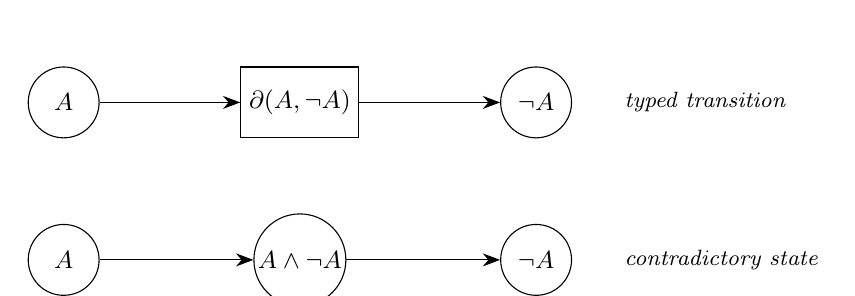
\begin{tikzpicture}[
  font=\small,
  state/.style={draw, circle, minimum size=9mm, inner sep=1pt},
  iface/.style={draw, rectangle, minimum width=15mm, minimum height=9mm, inner sep=2pt},
  arr/.style={-{Stealth[length=2.2mm]}}
]
\node[state] (A1) at (0,0)    {$A$};
\node[iface] (I)  at (3,0)    {$\partial(A,\neg A)$};
\node[state] (nA1) at (6,0)   {$\neg A$};
\draw[arr] (A1) -- (I);
\draw[arr] (I) -- (nA1);
\node[anchor=west, font=\footnotesize\itshape] at (7.0,0) {typed transition};

\node[state] (A2) at (0,-2)   {$A$};
\node[state] (M)  at (3,-2)   {$A \wedge \neg A$};
\node[state] (nA2) at (6,-2)  {$\neg A$};
\draw[arr] (A2) -- (M);
\draw[arr] (M) -- (nA2);
\node[anchor=west, font=\footnotesize\itshape] at (7.0,-2) {contradictory state};
\end{tikzpicture}
\caption{Two representations of the instant of change. Above: this
book's continuation-interface, where the middle object is a
\emph{transition} --- a different type from the states it connects
(drawn as a different shape, because it is one). Below: Priest's
dialetheic account, where the middle object is a \emph{state} satisfying
both $A$ and $\neg A$. The disagreement is not over which truth value
the middle point receives; it is over whether the transition should be
represented as a state at all. Per this chapter's qualifier, neither
representation is claimed to be correct for every change.}
\label{fig:state-vs-transition}
\end{figure}

\textbf{If this holds formally, the payoff is sharp --- and needs an equally
sharp qualifier.} Should this distinction survive further scrutiny, it
suggests: a contradiction attributed to a state may sometimes indicate
that the formalism lacks an object representing the transition between
states, rather than indicating that the state itself is genuinely
overdetermined. But ``sometimes'' is doing real work in that sentence and
cannot be dropped. Part III spent four chapters establishing that
genuine gluts --- states legitimately supporting both a proposition and its
negation --- are not errors requiring elimination. This chapter's proposal
must not be read as a general strategy for explaining away every glut as
``really'' a missing transition object; that would undo Part III's central
result rather than complementing it. The honest claim is narrower: \emph{some}
contradictions attributed to states may be artifacts of a state-only
vocabulary lacking a transition object, and identifying which
contradictions are which --- genuine overdetermination versus a
missing-object artifact --- is exactly the kind of question this chapter
raises and does not settle.

\hypertarget{chapter-18-motion-without-contradictory-location}{%
\chapter*{Chapter 18 --- Motion Without Contradictory Location}
\addcontentsline{toc}{chapter}{Chapter 18 --- Motion Without Contradictory Location}
\markboth{Chapter 18 --- Motion Without Contradictory Location}{Chapter 18 --- Motion Without Contradictory Location}\label{chapter-18-motion-without-contradictory-location}}

This chapter puts RSVP to genuine argumentative work rather than treating
it as a source of illustrative vocabulary, and the correspondence stays
marked \textbf{Tension}, as the matrix already has it --- this chapter doesn't
try to resolve that rating.

\textbf{Two rival representations of motion.} Priest's Hegelian treatment
characterizes motion through contradictory occupancy: at the relevant
instant, a moving object is both at a location and not at that location,
which is how motion gets represented at all within a framework built from
static positional predicates evaluated instant by instant. RSVP offers a
different starting point entirely --- it already has a vector field \(v\),
so motion doesn't need to be reconstructed from a sequence of static
positions in the first place; it's represented dynamically from the
start:
\[(\Phi, v, S)_t \longmapsto (\Phi, v, S)_{t + \Delta t}.\]

\textbf{The question this actually raises.} Not ``which account is correct,''
but something more specific: do contradictory positional predicates
reveal something genuinely ontological about motion --- that motion really
does involve a kind of instantaneous self-contradiction --- or do they
reveal something merely \emph{inadequate} about representing motion using
static positional predicates alone, a limitation of the vocabulary rather
than a discovery about the world? RSVP's vector field doesn't answer this
question by fiat; it demonstrates that a coherent, contradiction-free
representation of motion is available once the representation is allowed
to include velocity as a primitive rather than trying to derive motion
from position sequences after the fact. Whether that shows Priest's
contradiction is dispensable, or merely shows one particular vocabulary
happens to avoid it, is the tension this chapter leaves standing.

\textbf{The backward connection to Chapter 16.} This sharpens rather than
merely echoes Chapter 16's thesis. If states are projections of
histories --- if what's available at an instant is a slice through a
continuation rather than a self-sufficient object --- then a
position-only representation at a single instant has \emph{already} discarded
exactly the information (velocity, direction, rate) needed to distinguish
``is located here'' from ``is moving through here.'' Priest's contradictory
occupancy may be less a fact about motion and more a symptom of asking a
state-only vocabulary a question it was never equipped to answer, given
that the same vocabulary was already shown, in Chapter 16, to be too thin
to carry identity across time either.

\hypertarget{chapter-19-time-memory-and-irreversibility}{%
\chapter*{Chapter 19 --- Time, Memory, and Irreversibility}
\addcontentsline{toc}{chapter}{Chapter 19 --- Time, Memory, and Irreversibility}
\markboth{Chapter 19 --- Time, Memory, and Irreversibility}{Chapter 19 --- Time, Memory, and Irreversibility}\label{chapter-19-time-memory-and-irreversibility}}

\textbf{What Chain of Memory is not being used for.} CoM formalizes reasoning
trajectories --- sequences of latent states an inferential process passes
through --- and this chapter does not derive a theory of physical time from
it. That would overreach in exactly the way this book has tried to avoid
elsewhere: CoM's trajectories are about how a reasoning process gets from
one cognitive state to another, not about the structure of time itself,
and treating the two as the same theory would be a category error, not a
correspondence.

\textbf{What CoM is used for instead: a narrower, real distinction.}
\[\text{instantaneous state} \neq \text{history-indexed state}.\]
Two states that are, at a given moment, indistinguishable in every
respect that a snapshot could capture can nonetheless have arrived by
different histories --- and those different histories can license
different continuations going forward, even though nothing about the
present moment, examined on its own, shows this. Memory, on this
account, is not simply extra information carried inside an otherwise
complete state. It can encode \emph{the path by which the state became
reachable}, which is a fact about the state's history, not a fact
addable to its instantaneous content without changing what kind of
object a ``state'' is taken to be.

\textbf{A route from Priest toward this book's irreversibility work, stated as
a route rather than an equivalence.} Priest's Spread Hypothesis and his
broader treatment of temporal flow are themselves attempts to give
content to something like ``the present moment is thicker than an
instant.'' This chapter's history-indexed-state distinction is a
different, narrower device aimed at a related target --- not offered as
the same theory in different notation, and not offered as a replacement
for Priest's account, but as a route toward this book's own
irreversibility material that happens to pass near Priest's territory
without claiming to arrive at the same destination.

\textbf{Where the Leibniz Continuity Condition tension belongs, finally.} A
discrete repair operation, \(A_t \to A_{t+1}\), can look like a
discontinuous jump at one descriptive level --- nothing between the two
states, an instantaneous replacement --- while being implemented, at a
finer level of description, by a continuous underlying trajectory that
the discrete description simply doesn't resolve. This chapter's job is to
ask, honestly, whether that distinction actually reconciles the Leibniz
Continuity Condition (change is continuous, no jumps) with this book's
discrete repair events, or whether it's merely a redescription that
doesn't touch the real disagreement. If a finer-grained continuous
trajectory really does underlie every discrete repair this book has
posited, the tension dissolves without either side having to give
ground. If it doesn't --- if some repairs are genuinely discontinuous even
under arbitrarily fine redescription --- the tension should be preserved
exactly as the correspondence matrix has kept it, rather than talked
away by an appeal to description-level relativity that hasn't actually
been shown to apply.

\hypertarget{the-arc-of-part-v-and-what-it-hands-to-part-vi}{%
\section{The arc of Part V, and what it hands to Part VI}\label{the-arc-of-part-v-and-what-it-hands-to-part-vi}}

Four chapters, one continuous progression: identity requires continuation
across states (Chapter 16); change introduces a transition object that
states alone don't contain (Chapter 17); motion requires dynamical
information absent from position predicates taken instant by instant
(Chapter 18); memory distinguishes histories that terminate in otherwise
identical states (Chapter 19). Each chapter, in turn, challenges the
sufficiency of an instantaneous state a little further, and the four
together support a thesis Part V can claim as its own:

\begin{quote}
A state does not contain all the structure required to explain its own
continuation.
\end{quote}

This is not merely a summary --- it's exactly what Part VI needs before its
machinery can be trusted. Once Part VI moves into local sections,
restriction maps, reconstruction, and gluing, there is now a stated
reason not to assume a section's pointwise values exhaust its semantics:
Part V has spent four chapters showing that assumption fails even for
single, non-localized states, well before any cover or gluing condition
enters the picture.

\textbf{Two debts to preserve explicitly for Part VI's final pass, not to
resolve here.} First, Part IV established three genuinely different
failure modes --- glut (overdetermination), incompatibility (compatibility
obstruction), and dispersion (persistence failure under coarse-graining)
--- and this book should resist deciding whether dispersion is ``really''
topology until Part VI's own machinery is on the table to test against.
If Chapter 23/24's proposed topology turns out unable to distinguish
refinement-instability from ordinary incompatibility, that's evidence the
topology needs more structure, not a license to identify the two
phenomena by definitional fiat. Second, and more general: the final Part
VI pass should function less as an occasion to add machinery and more as
a type-check across the whole book --- every occurrence of support,
construction, admissibility, accessibility, compatibility, repair,
persistence, transition, and obstruction, checked against every other
part, to make sure two notions this book worked to keep separate haven't
quietly collapsed back together somewhere along the way.

\hypertarget{status-of-this-draft}{%
\section{Status of this draft}\label{status-of-this-draft}}

Written to let disagreement stand where it's earned. Chapter 17's central
result is qualified as carefully as its payoff is stated --- ``sometimes,''
not ``always,'' and the reason that qualifier can't be dropped is spelled
out rather than left implicit. Chapter 18 keeps its Tension rating rather
than resolving it in either direction. Chapter 19 poses the LCC question
as a genuine either/or rather than assuming the reconciling answer.
Nothing in this part quietly redescribes Priest in this book's vocabulary
without either agreeing with him outright or stating a specific,
checkable point of departure --- which was the actual test this part was
supposed to be.

\part{VI: Local Logic and Global Obstruction}\label{part-vi-local-logic-and-global-obstruction}

\hypertarget{chapter-20-local-support-and-logical-regimes}{%
\chapter*{Chapter 20 --- Local Support and Logical Regimes}
\addcontentsline{toc}{chapter}{Chapter 20 --- Local Support and Logical Regimes}
\markboth{Chapter 20 --- Local Support and Logical Regimes}{Chapter 20 --- Local Support and Logical Regimes}\label{chapter-20-local-support-and-logical-regimes}}

A proposition is usually introduced as something that is simply true or
false, with the four-valued and gap-tolerant systems arriving later as
modifications to that starting point --- extra machinery bolted onto a
prior notion of truth value. This chapter takes the opposite route.
Truth values are not primitive here. They are read off something more
basic: what evidence is actually available for and against a claim.

\textbf{Support, not truth value, as the starting object.} Fix a proposition
\(p\) and a region \(U\) of whatever domain is under discussion --- a context,
an observational patch, a tile in the sense already established elsewhere
in this book. Rather than asking whether \(p\) is true at \(U\), ask two
separate questions: is there positive evidence for \(p\) at \(U\), and is
there negative evidence for \(p\) at \(U\)? These questions are independent
of one another --- nothing forces an answer to one to constrain the answer
to the other --- and that independence is the whole of what makes four
values rather than two arise naturally, without stipulation.

Formally, let \(\mathcal{E}^+(U)\) and \(\mathcal{E}^-(U)\) be free abelian
groups generated by the distinct evidential witnesses --- observations,
derivations, testimony --- available for and against \(p\) within \(U\)
respectively. A single patch's support is then the pair
\((e^+, e^-) \in \mathcal{E}^+(U) \times \mathcal{E}^-(U)\), and the
\textbf{support map}

\[q(e^+, e^-) = \begin{cases} N & e^+ = 0,\ e^- = 0 \\ T & e^+ \neq 0,\ e^- = 0 \\ F & e^+ = 0,\ e^- \neq 0 \\ B & e^+ \neq 0,\ e^- \neq 0 \end{cases}\]

reads off one of Belnap and Dunn's~\cite{belnap1977,dunn1976} four values --- Neither, True, False,
Both --- as a consequence of the support data, not as a starting
assumption. \(\mathbb{F} = \{N,T,F,B\}\), ordered by the information order
\(N \sqsubseteq T \sqsubseteq B\), \(N \sqsubseteq F \sqsubseteq B\) with \(T,F\)
incomparable, is a complete lattice, and this matters later; for now it
is enough to note that \(q\) is a genuine function of the underlying
evidence, and that a glut is simply what you get when both kinds of
evidence happen to be present. Nothing about tolerating contradiction has
been stipulated. The four values are a description of four possible
evidential situations, and Both is one of them, on exactly the same
footing as the other three.

\textbf{What this chapter does not yet ask.} Everything above is stated for a
single patch \(U\) in isolation. It says nothing about what happens when
two overlapping patches each report support for the same \(p\) --- whether
their evidence agrees, whether it should be expected to, or what follows
if it doesn't. That is a genuinely separate question, deferred entirely
to Chapter 21. Keeping it separate is not merely tidy exposition; the
distinction between what a single patch supports and what multiple
patches agree on turns out to be the load-bearing distinction of this
part of the book, and blurring it --- treating ``every patch says \(T\)'' and
``every patch says \(T\) for the same reason'' as the same fact --- is
precisely the mistake this book's formal apparatus is built to make
impossible to state by accident.

\begin{center}\rule{0.5\linewidth}{0.5pt}\end{center}

\hypertarget{chapter-21-compatibility-and-gluing}{%
\chapter*{Chapter 21 --- Compatibility and Gluing}
\addcontentsline{toc}{chapter}{Chapter 21 --- Compatibility and Gluing}
\markboth{Chapter 21 --- Compatibility and Gluing}{Chapter 21 --- Compatibility and Gluing}\label{chapter-21-compatibility-and-gluing}}

Chapter 20 fixed what a single patch supports. This chapter asks whether
neighboring patches' support for the same proposition is the \emph{same}
support --- and gets the answer from a much simpler place than it might
appear to require.

\textbf{The question, precisely.} Let \(\{U_i\}\) be a cover, and suppose each
patch \(U_i\) reports local evidence \(e^+_i \in \mathcal{E}^+(U_i)\) for
\(p\)'s positive case (symmetrically for \(e^-_i\)). Where two patches
overlap, restriction maps \(\rho_{U_{ij}, U_i}\) carry each patch's evidence
down to what's visible on the shared region \(U_{ij} = U_i \cap U_j\). The
question is whether \(\rho_{U_{ij},U_i}(e^+_i)\) and \(\rho_{U_{ij},U_j}(e^+_j)\)
agree, as elements of \(\mathcal{E}^+(U_{ij})\).

It is tempting, and was in fact this book's own first attempt, to reach
here for Čech cohomology and ask whether some class is nonzero in
\(H^1\). That reach is wrong, for a reason worth stating once, precisely,
so it need not be revisited: for any specific chosen tuple of local
sections \(s = (s_i)\), the comparison \(\delta s\) --- the collection of
pairwise differences on overlaps --- is by construction a coboundary, and
therefore trivial in cohomology, whether or not the \(s_i\) actually agree.
Asking ``do these particular witnesses match'' is answered directly by
whether \(\delta s\) itself is the zero cochain, not by any cohomology
class built from it. The right tool is simpler than the wrong one, not
more elaborate, and this chapter uses only the tool the question actually
needs.

\textbf{Coherence defect.} Define
\[\delta^+(p) = \big(\rho_{U_{ij},U_j}(e^+_j) - \rho_{U_{ij},U_i}(e^+_i)\big)_{ij}\]
as an element of the Čech 1-cochains of \(\mathcal{E}^+\) relative to the
cover, and \(\delta^-(p)\) symmetrically. Say the positive (respectively
negative) evidence for \(p\) is \textbf{polarity-coherent} across the cover when
\(\delta^+(p) = 0\) (respectively \(\delta^-(p) = 0\)): every pair of
overlapping patches is contributing the \emph{same} witnesses, not merely
witnesses that happen to license the same verdict.

\begin{figure}[htbp]
\centering
\begin{tikzpicture}[
  node distance=1.1cm,
  font=\small
]
\node (title1) {Gluing};
\node[below=0.5cm of title1] (s1) {$s_1$};
\node[right=1.6cm of s1] (s2) {$s_2$};
\node[below=0.9cm of $(s1)!0.5!(s2)$] (ov) {$s_1|_{U_{12}} = s_2|_{U_{12}}$};
\node[below=0.9cm of ov] (glued) {$s \in \mathcal{A}(U_1 \cup U_2)$};
\draw[-{Stealth[length=2mm]}] (s1) -- (ov);
\draw[-{Stealth[length=2mm]}] (s2) -- (ov);
\draw[-{Stealth[length=2mm]},double] (ov) -- (glued);

\begin{scope}[xshift=6.3cm]
\node (title2) {Information-preserving merge};
\node[below=0.9cm of title2] (T) {$T$};
\node[right=1.6cm of T] (F) {$F$};
\node[below=0.9cm of $(T)!0.5!(F)$] (Bv) {$B$};
\draw[-{Stealth[length=2mm]}] (T) -- (Bv);
\draw[-{Stealth[length=2mm]}] (F) -- (Bv);
\end{scope}
\end{tikzpicture}
\caption{Gluing (left) requires a matching family: local sections that
already agree on the overlap combine into a unique global section.
Information-preserving merge (right) requires no such agreement: an FDE
join can combine \emph{disagreeing} reports (positive-only and
negative-only) into $B$, retaining rather than discarding what conflicts.
These are different operations, not two names for one --- see the
retracted correspondence discussed below.}
\label{fig:gluing-vs-merge}
\end{figure}

\textbf{Two different senses of restriction.} The restriction maps used above
carry a modeling choice worth making explicit rather than leaving
implicit, since the two readings genuinely differ. Restriction can mean
plain domain restriction --- the same assignment, viewed on a smaller
region, nothing lost. Or it can mean projection with possible
information loss --- evidence available across the whole of \(U_i\) need not
remain reconstructible from \(V \subset U_i\) alone, if the witnessing
particulars live outside \(V\)'s own resources. The second reading is the
one under which the coherence defect is doing real epistemic work rather
than bookkeeping, and it is the reading this book adopts going forward:
restriction is a genuine act of observation-with-possible-loss, not a
notational convenience. Spatial restriction (the morphism \(\rho_{VU}\))
and epistemic refinement (an ordering of increasing information, as in
Kripke-style forcing~\cite{kripke1963}) are different things, and treating them as
interchangeable was an earlier error in this construction's history worth
naming so it does not recur silently.

\textbf{What this chapter still does not settle.} Coherence, as defined here,
says nothing about which FDE value the patches end up reporting. A
proposition can be perfectly polarity-coherent and still be a glut (every
patch agrees, using the same witnesses, that \(p\) is Both). A proposition
can be badly incoherent and still show no glut at all --- every patch might
independently report \(T\), using witnesses that don't match each other in
the slightest. Whether that combination is even possible, and what it
would mean, is Chapter 22's question, not this one's --- this chapter has
deliberately stopped at the evidence layer and gone no further.

\begin{center}\rule{0.5\linewidth}{0.5pt}\end{center}

\hypertarget{chapter-22-contradiction-is-not-obstruction}{%
\chapter*{Chapter 22 --- Contradiction Is Not Obstruction}
\addcontentsline{toc}{chapter}{Chapter 22 --- Contradiction Is Not Obstruction}
\markboth{Chapter 22 --- Contradiction Is Not Obstruction}{Chapter 22 --- Contradiction Is Not Obstruction}\label{chapter-22-contradiction-is-not-obstruction}}

Chapters 20 and 21 built two structures over the same local data: what a
patch supports (Chapter 20), and whether neighboring patches' support
coheres (Chapter 21). This chapter's claim is that these are not two
views of one fact. They are genuinely separate facts, capable of varying
independently --- and that independence, rather than any single dramatic
case of contradiction, is the central result of this part of the book.

\textbf{The merge.} Given a family of local reports \(\{q_i(p)\}\), define the
pointwise merge
\[\Sigma(p) = \bigvee_i q_i(p),\]
the join in \(\mathbb{F}\)'s information order. Because \(\mathbb{F}\) is a
complete lattice, this join always exists --- there is no family of local
reports the merge fails to combine. Two propositions about it settle what
``merging'' produces:

\begin{quote}
\textbf{Support-Merge Proposition.} \(\Sigma(p) = B\) if and only if some
patch in the family reports positive support and some patch (possibly
the same one) reports negative support. \(\Sigma(p) = N\) if and only if
every patch touching \(p\) reports \(N\).
\end{quote}

\begin{quote}
\textbf{Glut-Free Reconstruction Obstruction.} A pointwise glut-free common
extension of the family into \(\{N,T,F\}\) exists if and only if no
proposition collects both positive and negative support across the
family --- that is, iff \(\Sigma(p) \neq B\) for every \(p\).
\end{quote}

Both are purely combinatorial statements about \(q_i\)-values; neither
mentions the coherence defect from Chapter 21. That is not an oversight ---
it is the point. And a genuine asymmetry falls out of the merge that is
worth stating on its own: \(N\) merges with anything to return that thing
unchanged (\(N \vee x = x\)), so absence of evidence never itself obstructs
reconstruction. Only actually incompatible polar evidence does. Gluts and
gaps are not mirror images of one another, whatever FDE's fourfold
notation suggests at a glance: \textbf{a glut is incompatible polar evidence; a
gap is merely insufficient polar evidence.}

\textbf{Mutual Non-Determination Proposition.} Neither the coherence status
\((\delta^+(p), \delta^-(p))\) from Chapter 21 nor the merged value
\(\Sigma(p)\) from this chapter determines the other. The proof is a
four-cell construction, and its economy is the whole argument: a
two-patch cover with overlap \(U_{12}\) populates all four combinations
directly.

\emph{A note on continuity with Part III.} This is the same construction
Chapter 12 built at the level of distinct evidence sources rather than
cover-indexed patches --- \(M(p) = \bigvee_i s_i(p)\) there, \(\Sigma(p) = \bigvee_i q_i(p)\) here. The two aren't merely analogous; \(\Sigma\) \emph{is}
\(M\), specialized to the case where the sources \(s_i\) happen to be
indexed by a genuine cover with overlaps, which is exactly what licenses
asking the coherence question (\(\delta^\pm\)) that Chapter 12 had no
apparatus for and deliberately didn't attempt. The name change from \(M\)
to \(\Sigma\) marks that shift in structure, not a change in what the
operation does.

\begin{longtable}[]{@{}
  >{\raggedright\arraybackslash}p{(\columnwidth - 4\tabcolsep) * \real{0.3333}}
  >{\raggedright\arraybackslash}p{(\columnwidth - 4\tabcolsep) * \real{0.3333}}
  >{\raggedright\arraybackslash}p{(\columnwidth - 4\tabcolsep) * \real{0.3333}}@{}}
\toprule\noalign{}
\begin{minipage}[b]{\linewidth}\raggedright
\end{minipage} & \begin{minipage}[b]{\linewidth}\raggedright
\(\delta\) coherent
\end{minipage} & \begin{minipage}[b]{\linewidth}\raggedright
\(\delta\) incoherent
\end{minipage} \\
\midrule\noalign{}
\endhead
\bottomrule\noalign{}
\endlastfoot
\textbf{\(\Sigma(p) = T\)} & (a) both patches report \(T\) via the \emph{same} witness & (c) both patches report \(T\) via \emph{different}, non-matching witnesses \\
\textbf{\(\Sigma(p) = F\)} & (a\('\)) both patches report \(F\) via the \emph{same} witness & (c\('\)) both patches report \(F\) via \emph{different}, non-matching witnesses \\
\textbf{\(\Sigma(p) = B\)} & (b) both polarities individually coherent, genuinely in conflict & (d) conflicting \emph{and} internally incoherent \\
\end{longtable}

The \(T\)/\(F\) rows are genuinely separate cells, not mirror images assumed
free --- (a\('\)) sets \(e^-_1 = e^-_2 = v\) (a shared negative witness, no
positive evidence anywhere), giving \(\delta^- = 0\); (c\('\)) sets
\(e^-_1 = v_1 \neq v_2 = e^-_2\), giving \(\delta^- \neq 0\) while both patches
still report the same verdict \(F\). Both are built the same way (a) and
(c) were, not inferred from them. The \(B\) row already covers both
polarities by construction --- a glut requires both positive and negative
support present somewhere in the family, so (b) and (d) don't need
separate positive- and negative-side versions the way the non-glut rows
did. Six cells, all built, none left to symmetry. That every cell is
populated is the entire proof --- neither axis constrains the other,
because both are demonstrably free to vary while the other is held fixed.

\begin{figure}[htbp]
\centering
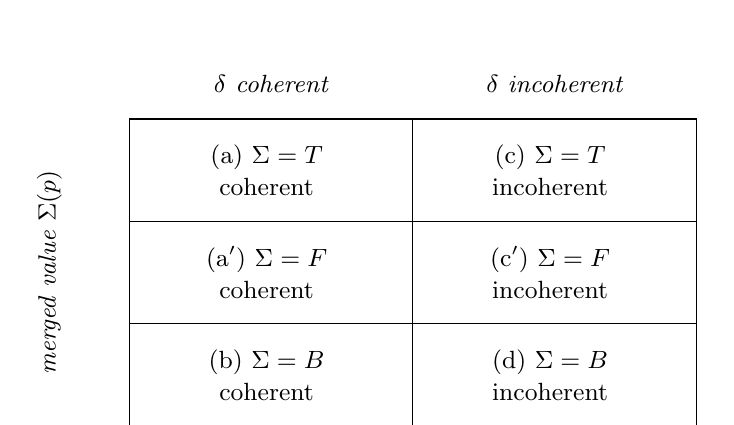
\begin{tikzpicture}[
  font=\small
]
\matrix (grid) [
  matrix of nodes,
  nodes={draw, minimum width=3.6cm, minimum height=1.3cm, align=center, anchor=center},
  row sep=-\pgflinewidth, column sep=-\pgflinewidth
] {
\shortstack{(a) $\Sigma=T$\\coherent} & \shortstack{(c) $\Sigma=T$\\incoherent} \\
\shortstack{(a$'$) $\Sigma=F$\\coherent} & \shortstack{(c$'$) $\Sigma=F$\\incoherent} \\
\shortstack{(b) $\Sigma=B$\\coherent} & \shortstack{(d) $\Sigma=B$\\incoherent} \\
};
\node[font=\small\itshape, above=0.2cm of grid-1-1.north, anchor=south] {$\delta$ coherent};
\node[font=\small\itshape, above=0.2cm of grid-1-2.north, anchor=south] {$\delta$ incoherent};
\node[font=\small\itshape, rotate=90, anchor=south] at ($(grid.west) + (-0.6,0)$) {merged value $\Sigma(p)$};
\end{tikzpicture}
\caption{The six realizability witnesses proving the Mutual
Non-Determination Proposition. Reading across a row: the same merged
value $\Sigma(p)$ occurs under both coherent and incoherent evidence.
Reading down a column: the same coherence status occurs under all three
merged values. Neither axis is a function of the other. Case (c) is the
one Priest's semantics alone cannot see: a classical-looking verdict
resting on evidence that does not actually agree with itself.}
\label{fig:mutual-non-determination}
\end{figure}

Case (b) is Priest's glut in its cleanest form: two well-founded,
internally coherent positions in genuine disagreement --- the positive case
coheres into one witness, the negative case coheres into a different one,
and they simply conflict. Call this the \textbf{clean glut}. Case (d) is the
same conflict compounded by internal incoherence on at least one side ---
part of what looks like cross-polarity disagreement may really be several
non-agreeing positive (or negative) sub-cases masquerading as one. Call
this the \textbf{confounded glut}. Both are legitimate uses of the word
``glut,'' and this book will keep them distinguished rather than treating
every \(\Sigma(p)=B\) as the same kind of event.

Case (c) deserves the most attention of the four, precisely because it is
the least dramatic. Nothing here looks unusual under FDE: both patches
say \(T\), no contradiction anywhere, nothing for a paraconsistent logic to
even notice. And yet the agreement is hollow in a specific, checkable
sense --- the patches are not agreeing about the same thing, only about the
same verdict. This is the case that carries the rest of Part VI, and it
recurs through Chapters 21 to 23 for that reason: it is the demonstration
that the support layer built in Chapters 20 and 21 is not decorative
machinery sitting underneath an otherwise complete four-valued logic. It
is detecting something four-valued logic alone cannot see at all.

\textbf{The headline result.} Contradiction, in Priest's sense, is a fact
about \(\Sigma(p)\). Obstruction to coherent reconstruction, in the sense
this book has been building since Chapter 21, is a fact about
\(\delta^\pm(p)\). This chapter's title is meant literally:
\textbf{contradiction is not obstruction.} A glut can be perfectly coherent. A
non-glut can be badly incoherent. Priest was right that gluts needn't
explode; this chapter's addition is that whether something needs
repairing at all cannot be read off \(\Sigma(p)\) in isolation --- which sets
up exactly the question Chapter 23 has to answer.

\begin{center}\rule{0.5\linewidth}{0.5pt}\end{center}

\hypertarget{chapter-23-repair-and-reconstruction}{%
\chapter*{Chapter 23 --- Repair and Reconstruction}
\addcontentsline{toc}{chapter}{Chapter 23 --- Repair and Reconstruction}
\markboth{Chapter 23 --- Repair and Reconstruction}{Chapter 23 --- Repair and Reconstruction}\label{chapter-23-repair-and-reconstruction}}

The progression through this part of the book has been

\[\text{support (Ch. 19)} \to \text{coherence (Ch. 20)} \to \text{non-determination (Ch. 21)} \to \text{repair (this chapter)}.\]

Chapter 22 established that support and coherence are independent facts.
This chapter asks what a repair operator does with both of them at once
--- and the answer is that it needs a third term it didn't previously have.

\textbf{Why case (c) cannot be folded into existing repair cost.} This book's
repair theory already has a cost formulation, \(E(a) + \lambda R(a)\),
where \(E\) is the ordinary cost of an action \(a\) and \(R\) is the cost of
repairing a polarity conflict --- a glut. Case (c) from Chapter 22 has
\(R(a) = 0\), exactly and correctly: there is no glut, no polarity conflict
of any kind, both patches agree \(p\) is \(T\). Whatever case (c) costs, it
is not a repair cost in the sense \(R\) was built to capture, and treating
it as one would erase the very distinction Chapters 21 and 22 exist to
establish.

\textbf{The third term.} Repair cost needs

\[J(a) = E(a) + \lambda R(a) + \mu C(a),\]

where \(C(a,p)\) is \textbf{coherence liability} --- the cost an action incurs
from depending on evidence that failed to cohere at Chapter 21's level,
even when Chapter 22's merge saw nothing wrong. Crucially, \(C\) cannot be
a fixed function of the coherence defect alone:

\[C(a,p) = \rho_a\big(\delta^+(p), \delta^-(p)\big),\]

action-relative by construction. The coherence defect is an objective
structural fact about the evidence configuration, unchanged by anyone's
plans; \(\rho_a\) is where the actual liability lives, and it depends on
what the action in question needs from the evidence.

A bridge reported open by camera evidence in one context and by
traffic-authority report in another is a witness mismatch --- but for an
action like \emph{drive across}, that mismatch is corroboration, not
incoherence: two independent reasons for the same conclusion. The same
structural fact, applied to an action like \emph{use this credential} where
the two contexts' positive evidence for ``the key is valid'' trace to two
different underlying keys, is disqualifying --- the action needs the
witnesses to be identical, not merely to agree on a verdict. Same
\(\delta^+(p) \neq 0\), opposite consequence, depending entirely on what the
action depends on. This is why \(\rho_a\) cannot be dispensed with in favor
of a single fixed penalty function: the liability is a fact about the
action's relationship to the evidence, not a fact about the evidence
alone.

\textbf{What this buys.} Under the old two-term functional, an action relying
on case (c)'s proposition is indistinguishable from one relying on case
(a) whenever their ordinary costs are equal --- neither has a glut, so
\(R = 0\) for both, and \(E + \lambda R\) has nothing left to compare. Under
the three-term functional, a witness-sensitive action pays through \(C\)
where a witness-insensitive one does not, even though \(\Sigma(p) = T\)
identically for both:

\begin{quote}
Two states indistinguishable under the FDE polarity merge can induce
different action preferences once evidential coherence enters the
decision functional.
\end{quote}

Which gives this part of the book its actual thesis, stated plainly:
\textbf{logical agreement does not imply evidential coherence, and rational
action may depend on both independently.} It is case (c), not the
dramatic glut cases, that earns the extra machinery its place --- a
classical-looking, contradiction-free agreement can still be the wrong
thing to act on, for reasons a four-valued semantics alone has no way to
express.

\textbf{A deliberate incompleteness.} This chapter does not commit to a
canonical form for \(\rho_a\) beyond the minimal binary flag --- sensitive or
insensitive --- used in the bridge/credential contrast above. That is a
choice, not a gap: establishing that an action-relative coherence
liability distinguishes configurations invisible to the old functional is
the result this chapter needs, and it holds regardless of which
particular metric or coefficient structure eventually fills in \(\rho_a\).
Committing to a graded, numerical version now would answer a question
this chapter hasn't yet earned the right to ask --- whether \(\rho_a\) should
depend on \emph{which} witness-identity condition an action needs, and how \(C\)
should aggregate across actions depending on several propositions at
once, are left open for exactly that reason.

\begin{center}\rule{0.5\linewidth}{0.5pt}\end{center}

\hypertarget{status-of-this-draft}{%
\section{Status of this draft}\label{status-of-this-draft}}

Written sequentially, as a test of whether the five revisions of scratch
work compose without the correction history as scaffolding. They do. The
mirror-case gap flagged in the first pass --- \(\Sigma(p) = F\) under each
coherence status, previously asserted by symmetry rather than built --- is
now closed with explicit constructions (a\('\)) and (c\('\)) added to Chapter
21's table. The progression from support to coherence to non-determination
to repair holds together as stated, case (c) does the work across three
chapters that it was meant to, and Chapter 23's deliberate incompleteness
around \(\rho_a\) is the honest state of that question rather than a
placeholder for something already decided.

\hypertarget{chapter-24-the-geometry-of-logical-regimes}{%
\chapter*{Chapter 24 --- The Geometry of Logical Regimes}
\addcontentsline{toc}{chapter}{Chapter 24 --- The Geometry of Logical Regimes}
\markboth{Chapter 24 --- The Geometry of Logical Regimes}{Chapter 24 --- The Geometry of Logical Regimes}\label{chapter-24-the-geometry-of-logical-regimes}}

Chapters 20 through 23 built three things over each proposition and each
cover: a support configuration (Chapter 20), a coherence defect on that
configuration (Chapter 21), and a repair cost that depends on both at
once (Chapter 23), with Chapter 22 establishing that the first two vary
independently. What hasn't been asked yet is what kind of \emph{space} all of
this lives in --- and whether calling it a geometry, rather than merely a
list of cases, is earned or aspirational. This chapter argues it's
earned, in one precise sense, and proposes the rest as a program rather
than claiming more than has been built.

\hypertarget{whats-actually-rigorous-t-f-b-n-as-fibers-not-points}{%
\section{1. What's actually rigorous: T, F, B, N as fibers, not points}\label{whats-actually-rigorous-t-f-b-n-as-fibers-not-points}}

Fix a cover \(\{U_i\}\) and a proposition \(p\). Define the \textbf{support-coherence
space} for \(p\),
\[\mathcal{S}(p) = \Big\{ \big(e^+_i, e^-_i\big)_i \ \Big|\ e^+_i \in \mathcal{E}^+(U_i),\ e^-_i \in \mathcal{E}^-(U_i) \Big\},\]
the set of all possible support assignments across the cover --- the full
data Chapter 20 works with, before anything is merged or compared. There
is a projection
\[\pi : \mathcal{S}(p) \to \mathbb{F}, \qquad \pi\big((e^+_i,e^-_i)_i\big) = \Sigma(p) = \bigvee_i q(e^+_i,e^-_i),\]
Chapter 22's merge. Chapter 22's central result, restated in this
chapter's terms, is that \(\pi^{-1}(T)\) is not a point --- it contains both
case (a) (coherent) and case (c) (incoherent), which are different
elements of \(\mathcal{S}(p)\) that happen to share an image under \(\pi\).
The same holds for every fiber. This is what it means, precisely rather
than suggestively, to say that \(T\), \(F\), \(B\), \(N\) are \textbf{coarse
projections of regions in a richer space}, not native points of the
space itself. Nothing here needed new machinery --- it's Chapter 22's
result, restated as a fact about a map between two spaces rather than as
a fact about two separately-computed quantities. That restatement is the
whole of what's rigorous in this chapter; everything past this section is
proposed rather than proven.

\hypertarget{why-a-taxonomy-isnt-yet-a-geometry}{%
\section{2. Why a taxonomy isn't yet a geometry}\label{why-a-taxonomy-isnt-yet-a-geometry}}

A taxonomy sorts \(\mathcal{S}(p)\) into labeled bins --- clean glut,
confounded glut, coherent-\(T\), incoherent-\(T\), and so on, exactly as
Chapter 22's six-cell table does. A geometry needs more: a notion of which
configurations are \emph{near} which others, and what it costs to move from
one to another. Without that, ``the space of logical regimes'' is a
figure of speech for a partition, and the chapter's title would be false
advertising. Two candidate structures are worth taking seriously, and
this is where TARTAN stops being a correspondence-matrix entry from an
earlier chapter and becomes load-bearing.

\hypertarget{neighborhoods-from-refinement-the-proposed-topology}{%
\section{3. Neighborhoods from refinement --- the proposed topology}\label{neighborhoods-from-refinement-the-proposed-topology}}

\(\mathcal{S}(p)\) as defined above is relative to one fixed cover
\(\{U_i\}\). TARTAN's recursive tiling gives a \emph{family} of covers, ordered
by refinement --- each tile decomposable into finer sub-tiles, with the
TARTAN Admissibility Theorem guaranteeing that global admissibility
reduces to tile-local admissibility at every level of that refinement,
not just at one chosen resolution. This suggests treating \(\mathcal{S}(p)\)
not as fixed to one cover but as assembled from the whole refinement
diagram --- coarser covers give coarser support-coherence spaces, finer
covers give finer ones, and the refinement maps between them are exactly
what a topology on the assembled space would need to be built from:
two configurations count as \emph{near} each other if they agree at some
coarse level of tiling and only differ once the tiling is refined past
some threshold.

This is proposed, not built. What would need proving: that refining a
cover is compatible with the coherence defect in the right way (does
refining a tile ever \emph{manufacture} an apparent coherence defect that
wasn't real at the coarser resolution, or only ever reveal genuine ones
that coarseness had hidden?), and that the resulting limit or colimit
construction is well-behaved enough to actually deserve the name
topology rather than merely a directed system of unrelated spaces. Both
are real technical questions, not merely items to gesture past.

\textbf{Running Part IV's test against this proposal.} Chapter 15 posed a
specific question for whoever built this topology to answer, rather than
leaving the relationship between dispersion obstruction and this
chapter's program unresolved indefinitely: does the topology sketched
above contain enough structure to measure \emph{persistence} under
refinement, or only \emph{neighborhoods}? As stated, it's the latter --- ``near''
here means agreeing at some coarse level and differing only past a
refinement threshold, which is a qualitative nearness relation with no
attached magnitude. Nothing in §3 as written could represent an
accumulation of small displacements the way Chapter 15's
\(\sum_i \epsilon_i\) does; there's no metric, uniformity, or filtration
here, only a directed system of covers. So the answer to Chapter 15's
test is settled, at least for this proposal in its current form:
\textbf{dispersion obstruction and this section's topology are not
duplicates.} This section, if built, would supply the qualitative
geometry --- which configurations are near which, at what refinement
depth. Dispersion needs the further scale structure Chapter 15
introduced on top of that, not in place of it. Whether this topology
should be \emph{extended} with that structure, or whether dispersion is
better left as a separate functional layered over a topology that stays
qualitative, is a design choice for whoever builds this section
properly --- this note only settles that the two aren't secretly the same
thing.

\hypertarget{distance-from-repair-cost-the-proposed-metric}{%
\section{4. Distance from repair cost --- the proposed metric}\label{distance-from-repair-cost-the-proposed-metric}}

Chapter 23's functional \(J(a) = E(a) + \lambda R(a) + \mu C(a)\) was built
to price an action's dependence on a given support-coherence
configuration, not to measure distance between two configurations
directly. But the ingredients are close enough to a metric to name the
gap precisely: for two configurations \(s, s' \in \mathcal{S}(p)\), define
a candidate transition cost as the minimal repair expenditure
(\(\lambda R + \mu C\) terms, stripped of the action-specific \(E\)) needed
to move from one to the other --- turning a confounded glut into a clean
one, or eliminating a coherence defect entirely, has some cost, and nearby
configurations should be the ones reachable cheaply.

This is also proposed rather than built, and for a specific, nameable
reason: \(J\) as defined in Chapter 23 is a cost \emph{of an action}, relative to
what that action needs from \(p\). A genuine distance on \(\mathcal{S}(p)\)
would need a notion of repair cost that doesn't route through any
particular action --- something closer to \(\inf_a\) over all actions, or a
repair cost defined directly on configurations rather than borrowed from
\(C(a,p)\). Whether that infimum is well-behaved, and whether it satisfies
anything like a triangle inequality, is exactly the kind of question this
chapter can pose but not yet answer.

\hypertarget{what-the-geometry-would-buy-if-built}{%
\section{5. What the geometry would buy, if built}\label{what-the-geometry-would-buy-if-built}}

Supposing both of §3 and §4 could be made rigorous, the payoff is the
thing the whole book has been organized around: \textbf{logical regimes become
regions of \(\mathcal{S}(p)\), not a list of separately-specified formal
systems.} The classical regime is the region where \(\delta^\pm = 0\)
everywhere and \(\Sigma(p) \neq B\) for every \(p\) --- Chapter 22's Glut-Free
Reconstruction condition, read as a subset rather than a proposition.
The paraconsistent regime is the region admitting \(\Sigma(p) = B\) without
requiring \(\delta = 0\) to accompany it --- a strictly larger region,
containing the classical one as a sub-region rather than standing beside
it as an alternative. A relevant-logic-flavored regime would be the
region where \(C(a,p) > 0\) matters for enough actions that propagation
needs the \(\rho_a\)-sensitivity machinery from Chapter 23 to behave
sensibly at all --- not a separate logic bolted on, but a description of
where in \(\mathcal{S}(p)\) an agent's actions live.

If this works, it inverts the usual presentation this book set out to
avoid: instead of ``here is classical logic, and here are its
non-classical rivals,'' the picture becomes one space, with the historical
logics showing up as its more heavily-traveled or more easily-described
regions --- classical logic isn't a rival to paraconsistency, it's the
sub-region of \(\mathcal{S}(p)\) where paraconsistency's extra room happens
not to be needed.

\hypertarget{honest-status}{%
\section{6. Honest status}\label{honest-status}}

Section 1 is proven, in the sense that it restates an already-established
result in geometric language rather than adding new content. Sections 3
and 4 are a program, stated as specifically as this draft can manage
without doing the actual work: two genuine technical questions (does
refinement only ever reveal coherence defects, never manufacture them;
does an action-independent repair distance exist and satisfy a triangle
inequality) stand between ``proposed'' and ``built.'' Section 3 additionally
now carries a settled answer to the question Chapter 15 posed about it:
as proposed, this topology is qualitative-only and doesn't duplicate
dispersion obstruction, which needs scale structure this section doesn't
yet have. Section 5 is the vision the rest of the book has been
implicitly working toward, stated plainly so it can be checked against,
not claimed as delivered. This chapter does what it was supposed to do
on the plan set out earlier: it was generated by the pressure of the
chapters before it, asks questions those chapters make it possible to
ask precisely, and answers only the one Chapter 15 handed it a decision
procedure for.


\appendix
\part{Mathematical Appendices}
\chapter{FDE Support, Merge, and Glut-Free Reconstruction}
\label{app:fde-support-merge}

This appendix collects the finite support calculus used in Parts III and VI in one place. It adds no new philosophical claim; its purpose is to make explicit the definitions and elementary propositions on which Chapters 10, 12, 20, and 22 rely.

\section*{Signed support and the four values}
Fix a proposition $p$. Let positive and negative support be represented by two indicators
\[
\sigma^+(p),\sigma^-(p)\in\{0,1\}.
\]
Define the support-value map $q:\{0,1\}^2\to\mathbb F$ by
\[
q(0,0)=N,\qquad q(1,0)=T,\qquad q(0,1)=F,\qquad q(1,1)=B.
\]
Equip $\mathbb F=\{N,T,F,B\}$ with the information order
\[
N\sqsubseteq T\sqsubseteq B,\qquad N\sqsubseteq F\sqsubseteq B,
\]
with $T$ and $F$ incomparable. Thus $\mathbb F$ is a finite complete lattice and, in particular,
\[
T\vee F=B,\qquad N\vee x=x,\qquad B\vee x=B.
\]

The same construction may be made over evidential witness groups. If $\mathcal E^+(U)$ and $\mathcal E^-(U)$ are the positive and negative evidence groups on a region $U$, define
\[
q(e^+,e^-)=
\begin{cases}
N,&e^+=0,\ e^-=0,\\
T,&e^+\neq0,\ e^-=0,\\
F,&e^+=0,\ e^-\neq0,\\
B,&e^+\neq0,\ e^-\neq0.
\end{cases}
\]
The four-valued semantics is therefore read from two independent support coordinates rather than taken as primitive.

\section*{Information merge}
Let $s_1,\ldots,s_n$ be independent support reports about $p$. Define
\[
M(p)=\bigvee_{i=1}^n s_i(p).
\]
When the reports are indexed by patches of a cover, Chapter 22 writes the same operation as
\[
\Sigma(p)=\bigvee_i q_i(p).
\]
Hence $\Sigma=M$ after specialization to cover-indexed sources.

\paragraph{Proposition A.1 (Support--Merge).}
$M(p)=B$ if and only if the family collectively contains positive support and negative support for $p$. Moreover, $M(p)=N$ if and only if every report is $N$.

\paragraph{Proof.}
Write each report as a pair $(\sigma_i^+,\sigma_i^-)$. Join in the information order is coordinatewise Boolean disjunction, so
\[
M(p)=q\!\left(\bigvee_i\sigma_i^+,\ \bigvee_i\sigma_i^-\right).
\]
The result is $B$ exactly when both displayed coordinates are $1$, and is $N$ exactly when both are $0$. \hfill$\square$

\section*{Glut-free reconstruction}
Let $\mathbb F_{\neg B}=\{N,T,F\}$. A glut-free common extension of a family $\{s_i(p)\}$ is an element $u\in\mathbb F_{\neg B}$ such that $s_i(p)\sqsubseteq u$ for every $i$.

\paragraph{Proposition A.2 (Glut-Free Reconstruction Obstruction).}
A glut-free common extension exists if and only if $M(p)\neq B$.

\paragraph{Proof.}
If $M(p)\neq B$, then $M(p)\in\mathbb F_{\neg B}$ and, by the defining property of a join, every $s_i(p)\sqsubseteq M(p)$. Conversely, if $M(p)=B$, the family contains both polarities. Any common upper bound must therefore dominate both $T$ and $F$, whose least upper bound is $B$. No element of $\mathbb F_{\neg B}$ can do so. \hfill$\square$

This proposition makes the gap/glut asymmetry exact. $N$ is not an obstruction: $N\vee x=x$. A gap records insufficient polar evidence. A glut records jointly retained positive and negative support, and becomes an obstruction only relative to a reconstruction regime that excludes $B$.

\chapter{Covers, Coherence Defects, and Mutual Non-Determination}
\label{app:coherence-defects}

This appendix isolates the cover-level apparatus of Chapters 20--23. Its main purpose is to prevent three operations from being conflated:
\[
\text{restriction}\neq\text{gluing}\neq\text{merge/repair}.
\]

\section*{Evidence presheaves and restriction}
Let $X$ be a domain with cover $\mathcal U=\{U_i\}$. For each open region $U$, let $\mathcal E^+(U)$ and $\mathcal E^-(U)$ be abelian groups generated by positive and negative evidential witnesses. For $V\subseteq U$, let
\[
\rho_{V,U}^{\pm}:\mathcal E^{\pm}(U)\to\mathcal E^{\pm}(V)
\]
be restriction maps satisfying identity and composition. The intended reading in Part VI permits information loss under restriction: evidence available on $U$ need not remain reconstructible from $V$ alone.

For a chosen family $e_i^\pm\in\mathcal E^\pm(U_i)$, define the overlap defect
\[
(\delta^\pm e)_{ij}
=
\rho_{U_{ij},U_j}^{\pm}(e_j^\pm)
-
\rho_{U_{ij},U_i}^{\pm}(e_i^\pm),
\qquad U_{ij}=U_i\cap U_j.
\]
The family is polarity-coherent when $\delta^\pm e=0$.

\paragraph{Remark.}
$\delta e$ is a \v{C}ech $1$-cochain and, for a chosen $0$-cochain $e$, is a coboundary by construction. Consequently its cohomology class cannot diagnose whether these particular witnesses agree: $[\delta e]=0$ automatically whenever the ordinary cochain complex is defined. The relevant test here is the cochain-level equation $\delta e=0$, not nonvanishing of $H^1$.

\section*{Ordinary gluing versus information merge}
Ordinary sheaf gluing begins with a matching family,
\[
\rho_{U_{ij},U_i}(e_i)=\rho_{U_{ij},U_j}(e_j),
\]
and produces a global section restricting exactly to each local section. By contrast, the FDE information merge
\[
\Sigma(p)=\bigvee_i q_i(p)
\]
can combine reports that do not match. If one patch reports $T$ and another $F$, the merge returns $B$; it does not produce a section whose restrictions are simultaneously the original $T$ and $F$ reports. Merge is therefore an information-preserving repair operation, not ordinary sheaf gluing.

\section*{Mutual non-determination}
Let the semantic coordinate be the merged value $\Sigma(p)\in\{N,T,F,B\}$ and the coherence coordinate be whether $(\delta^+(p),\delta^-(p))$ vanishes.

\paragraph{Proposition B.1 (Mutual Non-Determination).}
Neither the merged FDE value nor the coherence status determines the other.

\paragraph{Proof by realizability.}
A two-patch cover suffices. For $\Sigma=T$, choose either a shared positive witness on the overlap (coherent) or two distinct positive witnesses that restrict differently (incoherent). The same construction with negative witnesses realizes coherent and incoherent cases with $\Sigma=F$. For $\Sigma=B$, choose positive and negative evidence whose respective witnesses agree across the overlap to obtain a coherent glut, or choose a mismatch in at least one polarity to obtain an incoherent glut. Thus fixing $\Sigma$ does not fix coherence. Conversely, coherent and incoherent configurations occur at several distinct merged values, so coherence does not fix $\Sigma$. \hfill$\square$

The proposition is the formal core of the book's claim that contradiction and obstruction are different coordinates. A glut can be coherent, and a classical-looking verdict can be evidentially incoherent.

\section*{Action-relative coherence liability}
Chapter 23 extends the repair functional from
\[
E(a)+\lambda R(a)
\]
to
\[
J(a)=E(a)+\lambda R(a)+\mu C(a),
\qquad
C(a,p)=\rho_a\bigl(\delta^+(p),\delta^-(p)\bigr).
\]
The dependence on $a$ is essential: witness mismatch can be corroborative for an action insensitive to witness identity and disqualifying for an action that requires identity of the underlying witness. Hence coherence defect is structural, while coherence liability is action-relative.

\chapter{Resolution Profiles and Dispersion}
\label{app:dispersion}

Part IV separates degree-valued semantics from FDE's evidential polarity and then adds resolution as an explicit parameter. This appendix records the minimal mathematical structure needed for that move.

\section*{Resolution profiles}
Let $(\Lambda,\preceq)$ index resolutions or scales, and let
\[
v_\lambda(p)\in V
\]
be the value assigned to proposition $p$ at resolution $\lambda$, where $V$ carries a distance or other quantitative comparison $d$. The value $v_\lambda(p)$ and the full profile
\[
\lambda\longmapsto v_\lambda(p)
\]
are distinct objects. Many-valued semantics alone supplies the former; interpreting the latter as resolution behavior is an additional modeling choice of this book.

For a finite refinement or coarsening chain
\[
\lambda_0\preceq\lambda_1\preceq\cdots\preceq\lambda_n,
\]
define local increments
\[
\epsilon_i=d\bigl(v_{\lambda_i}(p),v_{\lambda_{i+1}}(p)\bigr)
\]
and accumulated variation
\[
D_{0:n}(p)=\sum_{i=0}^{n-1}\epsilon_i.
\]

\paragraph{Proposition C.1 (Local Smallness Does Not Imply Global Persistence).}
For every $\varepsilon>0$ and every target displacement $L>0$, there are sufficiently long chains for which each $\epsilon_i<\varepsilon$ while $D_{0:n}(p)\ge L$.

\paragraph{Proof.}
Choose $n>L/\varepsilon$ and a profile with constant increment $L/n$. Then $L/n<\varepsilon$ while the accumulated variation is $n(L/n)=L$. \hfill$\square$

The proposition captures the mechanism used in Chapter 15's sorites analysis. No adjacent step need contain a contradiction or a coherence failure. Dispersion is instead the accumulation of individually small changes into macroscopic displacement.

\section*{Persistence and topology}
A persistence functional $\mathcal P[s]$ may be chosen to measure how much of a verdict survives along a refinement/coarsening trajectory. The manuscript deliberately leaves its canonical form open; one possible family of models takes $\mathcal P$ to decrease with accumulated variation $D_{0:n}$.

This requires more structure than a bare topology. A topology can specify neighborhoods and continuity, but does not by itself assign magnitudes to successive displacements or provide an additive accumulation law. Consequently the qualitative topology proposed in Chapter 24 and the dispersion mechanism of Chapter 15 are distinct but related: the former can organize nearness under refinement, while the latter additionally requires a metric, uniformity, filtration, persistence functional, or comparable quantitative structure.

The resulting separation is
\[
\boxed{\text{compatibility}\neq\text{continuity}\neq\text{persistence}.}
\]
Compatibility asks whether fixed local data agree. Continuity asks which configurations are nearby. Persistence asks whether repeated locally small displacement remains globally small.


\part{Correspondence Ledger}
\hypertarget{priest-flyxion-correspondence-ledger-rev.-4}{%
\chapter*{Priest-Flyxion Correspondence Ledger (rev. 4)}
\addcontentsline{toc}{chapter}{Priest-Flyxion Correspondence Ledger (rev. 4)}
\markboth{Priest-Flyxion Correspondence Ledger (rev. 4)}{Priest-Flyxion Correspondence Ledger (rev. 4)}\label{priest-flyxion-correspondence-ledger-rev.-4}}

The matrix's function changes here. It no longer records what looked
formally alike before drafting; it records what the finished six-part
draft actually established, chapter by chapter, against the manuscript
files themselves (all six parts are drafted and were checked directly for
this revision, not reconstructed from progress summaries). Four columns:
the proposed correspondence, where it was tested, its final status, and
the exact qualification or open obligation attached to that status.

\textbf{Status vocabulary, revised (rev. 4) to separate three things ``Bridge''
was doing at once:}
- \textbf{Direct --- established}: the chapter actually supplied the
translation, not just a resemblance.
- \textbf{Bridge}: the manuscript develops a substantive connection but
stops short of derivation, without pinning down one specific missing
step --- the gap is real but not yet nameable as a single result.
- \textbf{Open obligation}: the manuscript develops the connection far enough
to expose one specific, nameable missing result --- a proof, a
derivation, or a technical question stated precisely enough that
answering it would close the gap. Stronger than Bridge because the
debt is specific, not diffuse.
- \textbf{Tension --- retained}: a genuine disagreement, kept rather than
resolved, and not to be papered over later.
- \textbf{Rejected}: a plausible-sounding correspondence was investigated and
found to conflate two genuinely different structures. Stronger than
``None'' --- this is a negative result, not an absence of one.
- \textbf{Distinct but related}: two structures address the same territory
without being the same object; neither Direct nor Rejected fits.
- \textbf{None}: no useful correspondence found; rare enough not to need its
own section.
- \textbf{Unpursued} (excluded from the tables below, listed separately at
the end): proposed during planning, but no chapter ever tested it.
This is not a status the finished manuscript can be scored against ---
the manuscript simply doesn't contain an attempt. Keeping these in the
main tables alongside Bridge and Open obligation would misstate what
the ledger claims to record: status \emph{after drafting}, for material
that was actually drafted.

\begin{center}\rule{0.5\linewidth}{0.5pt}\end{center}

\hypertarget{part-i-logic-as-constraint}{%
\section{Part I --- Logic as Constraint}\label{part-i-logic-as-constraint}}

\begin{longtable}[]{@{}
  >{\raggedright\arraybackslash}p{(\columnwidth - 6\tabcolsep) * \real{0.2500}}
  >{\raggedright\arraybackslash}p{(\columnwidth - 6\tabcolsep) * \real{0.2500}}
  >{\raggedright\arraybackslash}p{(\columnwidth - 6\tabcolsep) * \real{0.2500}}
  >{\raggedright\arraybackslash}p{(\columnwidth - 6\tabcolsep) * \real{0.2500}}@{}}
\toprule\noalign{}
\begin{minipage}[b]{\linewidth}\raggedright
Correspondence
\end{minipage} & \begin{minipage}[b]{\linewidth}\raggedright
Tested in
\end{minipage} & \begin{minipage}[b]{\linewidth}\raggedright
Status
\end{minipage} & \begin{minipage}[b]{\linewidth}\raggedright
Qualification / open obligation
\end{minipage} \\
\midrule\noalign{}
\endhead
\bottomrule\noalign{}
\endlastfoot
Classical consequence ↔ admissibility at maximal strictness & Ch.1 & Direct --- established & Classical logic is R turned to maximal strictness in every direction, not a default. \\
Logical consequence as truth-preservation ↔ \(x \leadsto_R y\) & Ch.1 & Direct --- established & Same shape as the ordinary definition, with admissibility as the varying parameter. \\
Explosion ↔ unrestricted propagation closure & Ch.1, Ch.4 & Direct --- established & Explosion is a specific, substantive closure choice, not a logical necessity. \\
Lewis's argument for explosion ↔ repair cost formulation & Ch.1 & Open obligation & Named missing result: a formal derivation from \(E(a)+\lambda R(a)\), not yet supplied --- currently gestured at only. \\
\end{longtable}

\hypertarget{part-ii-worlds-and-admissibility}{%
\section{Part II --- Worlds and Admissibility}\label{part-ii-worlds-and-admissibility}}

\begin{longtable}[]{@{}
  >{\raggedright\arraybackslash}p{(\columnwidth - 6\tabcolsep) * \real{0.2500}}
  >{\raggedright\arraybackslash}p{(\columnwidth - 6\tabcolsep) * \real{0.2500}}
  >{\raggedright\arraybackslash}p{(\columnwidth - 6\tabcolsep) * \real{0.2500}}
  >{\raggedright\arraybackslash}p{(\columnwidth - 6\tabcolsep) * \real{0.2500}}@{}}
\toprule\noalign{}
\begin{minipage}[b]{\linewidth}\raggedright
Correspondence
\end{minipage} & \begin{minipage}[b]{\linewidth}\raggedright
Tested in
\end{minipage} & \begin{minipage}[b]{\linewidth}\raggedright
Status
\end{minipage} & \begin{minipage}[b]{\linewidth}\raggedright
Qualification / open obligation
\end{minipage} \\
\midrule\noalign{}
\endhead
\bottomrule\noalign{}
\endlastfoot
Possible worlds ↔ admissible states \(w \in \operatorname{Adm}(R)\) & Ch.5 & Direct --- established & Deliberately ontology-neutral; realism/actualism/Meinongian debate left open on purpose. \\
Kripke necessity ↔ single-parameter invariance & Ch.5 (provisional), Ch.6 (corrected) & \textbf{Rejected as originally framed}, replaced & The single-\(R\) box formula conflates admissibility and accessibility; Ch.6 splits them into \((R, \mathcal{R})\). The rejection is of the \emph{conflation}, not of necessity-as-invariance generally. \\
Normal modal systems (K, T, S4, S5) ↔ structural constraints on \(\mathcal{R}\) & Ch.6 & Direct --- established & Reflexivity/transitivity/symmetry imposed on \(\mathcal{R}\) specifically, leaving \(R\) untouched. \\
Non-normal worlds ↔ refusal & Ch.7 & \textbf{Rejected}, replaced by non-normal worlds ↔ state-indexed regime \(R_w\) & Refusal is a targeted, Level-3 decline of one transformation; non-normal worlds suspend the compositional evaluation rule itself --- a different structural level. The original Direct rating was vocabulary-matching, not a derivation. \\
Impossible worlds ↔ locally varying admissibility & Ch.7 & Direct --- established, with a downstream open obligation & \(R_w\) formalizes this cleanly at the level of single states; the obligation surfaces one part later (see Part V/VI section below), not here. \\
Inconsistency / impossibility / non-normality as one phenomenon & Ch.7, using Part III as control case & Rejected as a collapse; three independent axes established & ``Impossibility is indexed to a constraint regime; contradiction is indexed to support'' --- stated as this part's foundational sentence. \\
Strict implication, conditional logics ↔ admissibility transport \(p \Rightarrow_R q\) & Ch.8 & Open obligation & Named missing result: the transformation-selection rule Lewis's similarity ordering supplied has no replacement yet. \\
Distinguishability geometry ↔ Lewisian similarity spheres & Ch.8 & Open obligation & Chapter ends on a precisely stated question (can similarity be derived from admissibility geometry) rather than claiming the replacement --- a nameable research question, not a diffuse gap. \\
\end{longtable}

\hypertarget{part-iii-gaps-gluts-and-propagation}{%
\section{Part III --- Gaps, Gluts, and Propagation}\label{part-iii-gaps-gluts-and-propagation}}

*(Editorial note: the working title ``Gaps, Gluts, and Obstructions'' is
retired for this part. Part VI earned the right to use ``obstruction'' as
a technical term distinct from contradiction; using the same word in
Part III's own heading, before that distinction exists, would quietly
reinstate the association the later chapters worked hard to separate.
If the manuscript's actual Part III title still reads ``\ldots and
Obstructions,'' it should be changed to match.)

\begin{longtable}[]{@{}
  >{\raggedright\arraybackslash}p{(\columnwidth - 6\tabcolsep) * \real{0.2500}}
  >{\raggedright\arraybackslash}p{(\columnwidth - 6\tabcolsep) * \real{0.2500}}
  >{\raggedright\arraybackslash}p{(\columnwidth - 6\tabcolsep) * \real{0.2500}}
  >{\raggedright\arraybackslash}p{(\columnwidth - 6\tabcolsep) * \real{0.2500}}@{}}
\toprule\noalign{}
\begin{minipage}[b]{\linewidth}\raggedright
Correspondence
\end{minipage} & \begin{minipage}[b]{\linewidth}\raggedright
Tested in
\end{minipage} & \begin{minipage}[b]{\linewidth}\raggedright
Status
\end{minipage} & \begin{minipage}[b]{\linewidth}\raggedright
Qualification / open obligation
\end{minipage} \\
\midrule\noalign{}
\endhead
\bottomrule\noalign{}
\endlastfoot
Truth-value gaps ↔ underdetermination (absence of both polarities) & Ch.9 & Direct --- established & Gap is not a third truth value bolted on; it's what ``no answer yet'' already means once the two support questions are separated. \\
Truth-value gluts ↔ overdetermination (retained conflicting evidence) & Ch.10 & Direct --- established & Sharper than ``some propositions are both true and false'' --- contradictory evidence need not be deleted merely for conflicting. \\
FDE's four values ↔ independent \(\sigma^+,\sigma^-\) & Ch.9--10, sharpened again in Ch.20 & Direct --- established & Became the entry point into Part VI's sheaf machinery, not merely a tableaux gloss. \\
Disjunctive syllogism failure ↔ restricted propagation & Ch.11 & Direct --- established, technical centerpiece & DS's second step is shown to silently assume positive/negative support are mutually exclusive --- false exactly at overdetermined points. Not an ad hoc patch. \\
LPm / classical recapture ↔ repair biased toward consistency & Ch.12 & Direct --- established & Pays the cost of a glut only where evidence leaves no alternative; classical elsewhere. \\
FDE merge ↔ glut-free reconstruction obstruction & Ch.12, restated at cover level Ch.23 & Direct --- established, order-theoretic & Deliberately not cohomological in Part III; the cover-level generalization was checked for compatibility during Part VI's final pass and confirmed to be the same operation, not merely analogous (see Ch.23 row below). \\
Relevant logics (ternary relation) ↔ propagation licensing & Ch.11 gestures at it via the DS mechanism & Open obligation & Named missing result: expressive equivalence to the ternary relation, neither shown nor disproven. \\
\end{longtable}

\hypertarget{part-iv-construction-vagueness-and-degree}{%
\section{Part IV --- Construction, Vagueness, and Degree}\label{part-iv-construction-vagueness-and-degree}}

\begin{longtable}[]{@{}
  >{\raggedright\arraybackslash}p{(\columnwidth - 6\tabcolsep) * \real{0.2500}}
  >{\raggedright\arraybackslash}p{(\columnwidth - 6\tabcolsep) * \real{0.2500}}
  >{\raggedright\arraybackslash}p{(\columnwidth - 6\tabcolsep) * \real{0.2500}}
  >{\raggedright\arraybackslash}p{(\columnwidth - 6\tabcolsep) * \real{0.2500}}@{}}
\toprule\noalign{}
\begin{minipage}[b]{\linewidth}\raggedright
Correspondence
\end{minipage} & \begin{minipage}[b]{\linewidth}\raggedright
Tested in
\end{minipage} & \begin{minipage}[b]{\linewidth}\raggedright
Status
\end{minipage} & \begin{minipage}[b]{\linewidth}\raggedright
Qualification / open obligation
\end{minipage} \\
\midrule\noalign{}
\endhead
\bottomrule\noalign{}
\endlastfoot
Intuitionistic construction ↔ reconstruction path & Ch.13 & Direct --- established, sharpened & Pinned specifically to \(\neg\neg p \to p\) failing, not a looser ``existence from absurdity'' slogan --- the earlier looser version would have overstated the correspondence. \\
Support vs.~constructibility as one axis vs.~two & Ch.13 & Rejected as one axis; established as two orthogonal coordinates & A non-constructive derivation and a genuine construction can both count as positive support; Part III's apparatus doesn't (and didn't need to) distinguish them. \\
Many-valued/fuzzy degree ↔ resolution-stability & Ch.14 & Bridge, explicitly labeled as this book's added interpretation & Corrected from an earlier draft that stated this as though many-valued semantics already meant it. \(v_\lambda(p)\) vs.~the resolution profile \(\lambda \mapsto v_\lambda(p)\) now kept distinct. \\
Sorites / vagueness ↔ dispersion obstruction & Ch.15 & Bridge, developed & Corrected definition: accumulation of small variation, not exact-agreement-everywhere (\(\sum_i \epsilon_i\) need not be small even when each \(\epsilon_i\) is negligible). The earlier ``N and B both fail to fit \{T,F\}'' framing this traces back to is now understood to have been too coarse; superseded, not merely refined. \\
Dispersion obstruction ↔ Ch.24's proposed topology & Ch.15, tested directly against Ch.24 §3 during Part VI's final pass & \textbf{Distinct but related} & Ch.24's topology is qualitative-only (neighborhoods, no metric); dispersion needs the accumulation structure Ch.15 introduced. Confirmed by direct test, not assumed either way. \\
\end{longtable}

\hypertarget{part-v-identity-change-and-worldhood}{%
\section{Part V --- Identity, Change, and Worldhood}\label{part-v-identity-change-and-worldhood}}

\begin{longtable}[]{@{}
  >{\raggedright\arraybackslash}p{(\columnwidth - 6\tabcolsep) * \real{0.2500}}
  >{\raggedright\arraybackslash}p{(\columnwidth - 6\tabcolsep) * \real{0.2500}}
  >{\raggedright\arraybackslash}p{(\columnwidth - 6\tabcolsep) * \real{0.2500}}
  >{\raggedright\arraybackslash}p{(\columnwidth - 6\tabcolsep) * \real{0.2500}}@{}}
\toprule\noalign{}
\begin{minipage}[b]{\linewidth}\raggedright
Correspondence
\end{minipage} & \begin{minipage}[b]{\linewidth}\raggedright
Tested in
\end{minipage} & \begin{minipage}[b]{\linewidth}\raggedright
Status
\end{minipage} & \begin{minipage}[b]{\linewidth}\raggedright
Qualification / open obligation
\end{minipage} \\
\midrule\noalign{}
\endhead
\bottomrule\noalign{}
\endlastfoot
Necessary/contingent identity, rigid designation ↔ trajectory-first ontology & Ch.16 & Bridge & Explicitly not claimed to derive rigid designation --- rigid designation is the comparison case, not a target reduced to this book's account. \\
Identity ↔ invariant of admissible continuation & Ch.16 & Direct --- established, with one open dependency & The thesis itself is stated cleanly; but see the \(R_w\)/continuation row below --- this chapter's own notion of ``admissible'' is underspecified once regimes vary by state. \\
Priest's contradictory transition instant ↔ continuation-interface object & Ch.17 & Tension --- retained, as a productive alternative & Explicitly qualified ``sometimes, not always'' --- must not become a general argument against dialetheism, given Part III's four chapters on genuine gluts. Not a derivation of Priest's account; a rival with a named scope limit. \\
Hegelean motion ↔ RSVP field dynamics & Ch.18 & Tension --- retained & Not upgraded despite RSVP doing real argumentative work; the ontological-fact-vs-inadequate-vocabulary question is left open on purpose. \\
Leibniz Continuity Condition ↔ discrete repair events & Ch.19 & Tension --- retained, given a specific test & ``Does a continuous trajectory underlie every discrete repair at some finer description'' is posed as a real either/or, not assumed to reconcile. \\
Spread Hypothesis / temporal flow ↔ Chain of Memory & Ch.19 & Bridge, deliberately narrowed & Explicitly not a theory of physical time --- narrowed to instantaneous-state ≠ history-indexed-state. Overselling this was an identified risk and avoided. \\
\textbf{\(R_w\) (Ch.7) ↔ admissible continuation (Ch.16)} & Ch.16, surfaced during Part VI's final pass & \textbf{New open research problem --- not resolved during reconciliation, on purpose} & \(x_{t} \xrightarrow{?} x_{t+1}\) with \(R_{x_t} \neq R_{x_{t+1}}\): ``admissible continuation'' doesn't yet say relative to which regime a transition step is judged --- \(R_{x_t}\), \(R_{x_{t+1}}\), an intersection/union, a transport of one into the other, or a distinct transition regime \(R_\gamma\). Ch.17's transition-as-its-own-type move suggests the last option but was correctly not promoted to a definition. This is a genuine result of completing all six parts, not a loose end to patch quietly. \\
\end{longtable}

\hypertarget{part-vi-local-logic-and-global-obstruction}{%
\section{Part VI --- Local Logic and Global Obstruction}\label{part-vi-local-logic-and-global-obstruction}}

\begin{longtable}[]{@{}
  >{\raggedright\arraybackslash}p{(\columnwidth - 6\tabcolsep) * \real{0.2500}}
  >{\raggedright\arraybackslash}p{(\columnwidth - 6\tabcolsep) * \real{0.2500}}
  >{\raggedright\arraybackslash}p{(\columnwidth - 6\tabcolsep) * \real{0.2500}}
  >{\raggedright\arraybackslash}p{(\columnwidth - 6\tabcolsep) * \real{0.2500}}@{}}
\toprule\noalign{}
\begin{minipage}[b]{\linewidth}\raggedright
Correspondence
\end{minipage} & \begin{minipage}[b]{\linewidth}\raggedright
Tested in
\end{minipage} & \begin{minipage}[b]{\linewidth}\raggedright
Status
\end{minipage} & \begin{minipage}[b]{\linewidth}\raggedright
Qualification / open obligation
\end{minipage} \\
\midrule\noalign{}
\endhead
\bottomrule\noalign{}
\endlastfoot
Local valuations ↔ local admissible sections \(s_i \in \mathcal{A}(U_i)\) & Ch.20 & Direct --- established & \\
Compatibility of local descriptions ↔ Čech coboundary vanishing & Ch.21 & Direct --- established, corrected apparatus & Not literal \(H^1\): for any chosen 0-cochain, \(\delta s\) is a coboundary by construction, so its class in \(H^1\) is trivially zero regardless of agreement. Renamed \textbf{coherence defect} \(\delta^\pm(p) \in \check{C}^1\), a cochain-level check. \\
Failure of global coherent determination ↔ nonzero \(H^1\) / glut & Ch.20--22 & \textbf{Rejected as originally stated}, replaced by the Mutual Non-Determination Proposition & ``Glut \(= [g] \neq 0\)'' is not a valid identification --- glut is semantic (dual support), \(H^1\)-type obstruction is geometric. The corrected result: coherence status and the FDE merge \(\Sigma(p)\) determine neither each other, proven by an explicit six-cell realizability table (Ch.22), not asserted by analogy. \\
Bilattice join ↔ ordinary sheaf gluing & Ch.20--21 & \textbf{Rejected} & Join is an information-preserving merge/repair of a non-matching family; gluing requires a family that already agrees on overlaps. Different operations under the same informal word ``combine.'' Terminology fixed going forward: restriction ≠ gluing ≠ repair. \\
TARTAN ↔ local-to-global logical regime assembly & Ch.24 §3 (proposed) & Open obligation & Two named missing results: does refinement only reveal genuine coherence defects or manufacture spurious ones; is the resulting limit/colimit well-behaved. \\
Ch.12's merge \(M\) ↔ Ch.23's merge \(\Sigma\) & Ch.23, checked directly during Part VI's final pass & Direct --- identified & \(\Sigma = M\) under cover indexing; the name change marks the structural generalization (bare sources → cover-indexed patches), not a different operation. \\
\(T,F,B,N\) ↔ fibers of a projection, not points of a richer space & Ch.24 §1 & Direct --- established & A restatement of the Mutual Non-Determination Proposition in geometric language, not new content --- the only fully rigorous claim in Ch.24. \\
Repair cost as a metric on \(\mathcal{S}(p)\) & Ch.24 §4 (proposed) & Open obligation & Two named missing results: whether an action-independent repair distance exists, and whether it satisfies a triangle inequality. \\
\end{longtable}

\begin{center}\rule{0.5\linewidth}{0.5pt}\end{center}

\begin{center}\rule{0.5\linewidth}{0.5pt}\end{center}

\hypertarget{unpursued-correspondences}{%
\section{Unpursued correspondences}\label{unpursued-correspondences}}

Two entries inherited from the original planning-stage matrix never had
a chapter written for them. They are not weak Bridges or exposed
obligations --- the manuscript contains no attempt to test them at all,
and listing them in the main tables above would misstate what this
ledger claims to record (status \emph{after drafting}, for material the
finished six parts actually contain).

\begin{longtable}[]{@{}
  >{\raggedright\arraybackslash}p{(\columnwidth - 4\tabcolsep) * \real{0.3333}}
  >{\raggedright\arraybackslash}p{(\columnwidth - 4\tabcolsep) * \real{0.3333}}
  >{\raggedright\arraybackslash}p{(\columnwidth - 4\tabcolsep) * \real{0.3333}}@{}}
\toprule\noalign{}
\begin{minipage}[b]{\linewidth}\raggedright
Correspondence
\end{minipage} & \begin{minipage}[b]{\linewidth}\raggedright
Original proposal
\end{minipage} & \begin{minipage}[b]{\linewidth}\raggedright
Why it stayed unpursued
\end{minipage} \\
\midrule\noalign{}
\endhead
\bottomrule\noalign{}
\endlastfoot
Priest's semantic closure (self-referential truth predicate) ↔ Spherepop's history-based operational semantics & A self-referential object language and a computation model that can refer to its own prior states looked structurally similar & No chapter in Parts I--VI was assigned this topic; the six-part outline never routed through it \\
Priest's naive/paraconsistent set theory (material, relevant, and model-theoretic strategies) ↔ obstruction as candidate propagation rules & Priest's three strategies for handling set-theoretic paradoxes looked like candidate instances of this book's propagation-restriction machinery & Same reason --- no chapter's scope included it \\
\end{longtable}

This isn't a defect in the finished book. A twenty-four-chapter argument
built around one central hierarchy doesn't need to absorb every topic
Priest covers across two books, and both of these are now more
approachable than they would have been before this project's framework
existed --- they're candidates for separate future work precisely because
the machinery to attempt them properly (the support/coherence/repair
apparatus, the admissibility regime vocabulary) now exists in a form
mature enough not to require inventing it from scratch alongside the
comparison itself.

\begin{center}\rule{0.5\linewidth}{0.5pt}\end{center}

\hypertarget{what-changed-as-a-record-rather-than-a-silent-overwrite}{%
\section{What changed, as a record rather than a silent overwrite}\label{what-changed-as-a-record-rather-than-a-silent-overwrite}}

Three correspondences were investigated and found to conflate distinct
structures, and are marked Rejected rather than quietly dropped: glut as
a nonzero cohomology class, bilattice join as ordinary sheaf gluing, and
non-normal worlds as refusal. All three were plausible enough to have
been rated Direct or treated as settled before the relevant chapter was
actually drafted. That they didn't survive contact with the chapters is
evidence the drafting process constrained its own conclusions rather than
rationalizing whatever correspondence was proposed first.

One new open research problem --- the \(R_w\)/continuation transition rule ---
was generated by completing Parts II and V, not resolved by their
completion. It's recorded here deliberately unresolved, per instruction,
since fixing it during this reconciliation pass would erase evidence that
finishing the book found a real gap rather than merely filling in a
pre-drawn outline.

This ledger is now the right basis for the book's introduction and
conclusion, and for identifying which individual results (the Mutual
Non-Determination Proposition and its realizability proof, most likely,
along with the \(R_w\)/continuation problem) might warrant a standalone
paper ahead of the full manuscript.

\textbf{This revision's specific change}: split the undifferentiated Bridge
category into Bridge (diffuse gap) and Open obligation (one nameable
missing result), reclassifying five rows accordingly, and moved the two
correspondences the manuscript never actually tested (semantic
closure/Spherepop, naive set theory) out of the main tables into their
own section. The ledger's claim to record what the finished manuscript
established was slightly inconsistent with carrying two rows the
manuscript never attempted; that inconsistency is now fixed rather than
carried forward again.


\backmatter
\chapter*{References}
\addcontentsline{toc}{chapter}{References}
\begin{thebibliography}{99}

\bibitem{belnap1977}
Belnap, N.~D. (1977). A useful four-valued logic. In J.~M. Dunn and G.~Epstein (Eds.), \emph{Modern Uses of Multiple-Valued Logic} (pp.~5--37). Dordrecht: Reidel.

\bibitem{dunn1976}
Dunn, J.~M. (1976). Intuitive semantics for first-degree entailments and `coupled trees'. \emph{Philosophical Studies}, 29, 149--168.

\bibitem{heyting1956}
Heyting, A. (1956). \emph{Intuitionism: An Introduction}. Amsterdam: North-Holland.

\bibitem{kripke1963}
Kripke, S.~A. (1963). Semantical analysis of modal logic I: Normal modal propositional calculi. \emph{Zeitschrift f\"ur Mathematische Logik und Grundlagen der Mathematik}, 9, 67--96.

\bibitem{lewis1973}
Lewis, D. (1973). \emph{Counterfactuals}. Oxford: Blackwell.

\bibitem{lukasiewicz1920}
{\L}ukasiewicz, J. (1970). On three-valued logic. In L.~Borkowski (Ed.), \emph{Selected Works} (pp.~87--88). Amsterdam: North-Holland. (Original work published 1920.)

\bibitem{priest2006}
Priest, G. (2006). \emph{In Contradiction: A Study of the Transconsistent} (Expanded ed.). Oxford: Clarendon Press.

\bibitem{priest2008}
Priest, G. (2008). \emph{An Introduction to Non-Classical Logic: From If to Is} (2nd ed.). Cambridge: Cambridge University Press.

\end{thebibliography}

\end{document}
